\documentclass[12pt, a4paper]{article}
\usepackage{caption}
\usepackage{graphicx}
\usepackage{amsmath, amsfonts, amssymb, amsthm}
\usepackage{xcolor}
\usepackage{listings}
\usepackage{hyperref}
\usepackage{tikz}
\usetikzlibrary{positioning, quotes}
\counterwithin*{equation}{subsection}
\title{Logiske udsagn}
\date{2021}
\author{Kristoffer Klokker}
\begin{document}
	\maketitle
	\clearpage
	\tableofcontents
	\clearpage
		\section{Logiske udsagn}
			Proposition - is a declarative sentence, either true or false.\\
			Senitial variables - variables presenting propositions, most used letters: $p,q,r,s$\\
			True propositions are denoted $T$ and false are denoted $F$\\
			Atomic propositions - the most simple version of a proposition\\

		\section{Logiske operatore - 1/9/2021}
			Tegn | navn | betydning\\
			$\neg$ | negation | Invers\\
			$\land$ | conjuction| Og\\
			$\lor$ | disjunction| Eller\\
			$\rightarrow$ | conditional | Implementere\\
			$\iff$ | biimplimentation | To ens udtryk\\
			$\oplus$ Exclusive or / XOR | sand ved én sand\\
			Præcedens hieraki: $\neg \land \lor \rightarrow \iff$\\
			$\oplus$ har ikke en specifik plads og derfor skal altid have parentes.
			\subsection{Logiske tabeller}
				Logiske tabeller kan bruges, til at overskueligegøre logiske udtryk.\\
				De kan også være til gavn for at ækvivalenser.\\
				\begin{table}[h!]
				\begin{tabular}{|l|l|}
				P & $\neg P$ \\
				S & F\\
				F & S                    
				\end{tabular}
				\end{table}
				\begin{table}[h!]
				\begin{tabular}{|l|l|l|l|}
				\hline
				P & Q & $P\land Q$ & $P \lor Q$ \\ \hline
				S & S & S                       & S                       \\ \hline
				S & F & F                       & S                       \\ \hline
				F & S & F                       & S                       \\ \hline
				F & F & F                       & F                       \\ \hline
				\end{tabular}
				\end{table}
			\subsection{Implimentation}
				$P\rightarrow Q$\\
				P hypotense/antagelse\\
				Q konklusion\\
				eks. $x>0 \rightarrow 2x \geq x$\\
				$x=1 \rightarrow s s$\\
				$x=0 \rightarrow f s$\\
				$x=-1 \rightarrow f f$\\
				I alle tre tilfælde er implikationen sand.\\
				\begin{table}[h!]
				\begin{tabular}{|l|l|l|}
				\hline
				P & Q & $P\rightarrow Q$ \\ \hline
				S & S & S                          \\ \hline
				S & F & F                          \\ \hline
				F & S & S                          \\ \hline
				F & F & S                          \\ \hline
				\end{tabular}
				\end{table}\\
				For the proposition $p\rightarrow q$ are the following:\\
					converse: $q\rightarrow p$\\
					Contrapositive: $\neg q \rightarrow \neg p$\\
					Inverse: $\neg p \rightarrow \neg q$\\
					example:\\
					The home team wins whenever it is raining.\\
					p = if it is raining\\
					q = then then home team wins\\
					converse: If the home team wins, then it is raining\\
					contrapositive: If the home team does not win, then it is not raining.\\
					inverse: If it is not raining, then the home team does not win.\\[5mm]
				eksempler på implikation.\\
					b: Du har købt en billet\\
					t: Du kan tage toget\\
					$b\rightarrow t$\\
					$\neg t \rightarrow \neg b$\\
					\begin{table}[h!]
					\begin{tabular}{|l|l|l|l|l|l|}
					\hline
					P & Q & $P\rightarrow Q$ & $\neg Q$ & $\neg P$ & $\neg Q \rightarrow \neg P$ \\ \hline
					S & S & S                          & F                     & F                     & S                                                                   \\ \hline
					S & F & F                          & S                     & F                     & F                                                                   \\ \hline
					F & S & S                          & F                     & S                     & S                                                                   \\ \hline
					F & F & S                          & S                     & S                     & S                                                                   \\ \hline
					\end{tabular}
					\end{table}
				Som det kan ses i tabellen ses det at $$P\rightarrow Q \equiv \neg P \rightarrow \neg Q$$\\
				Altså implikationen er ækvivalent til den negeriske implikation.
			\subsection{Bi implikation}
				$p\iff q$\\
				p og q har samme sandhedsværdi\\
				\begin{table}[h!]
				\begin{tabular}{|l|l|l|}
				\hline
				P & Q & $P\iff Q$ \\ \hline
				S & S & S                                 \\ \hline
				S & F & F                                 \\ \hline
				F & S & F                                 \\ \hline
				F & F & S                                 \\ \hline
				\end{tabular}
				\end{table}
				Bliver kaldt hviss/iff\\
				$P\iff Q \equiv (P\rightarrow Q) \land (Q\rightarrow P)$\\
			\subsection{Exclusive or / XOR}
				$P \oplus Q$\\
				P og Q har forskellgie sandhedsværider\\
				\begin{table}[h!]
				\begin{tabular}{|l|l|l|}
				\hline
				P & Q & $P\oplus Q$ \\ \hline
				S & S & F                         \\ \hline
				S & F & S                         \\ \hline
				F & S & S                         \\ \hline
				F & F & F                         \\ \hline
				\end{tabular}
				\end{table}
			\subsection{Ydeligere ækvivalenser}
				Compound proposition - a collection of logic operators\\
				Tautology - an always true compound $p\lor \neg p$\\
				Contradiction - an always false compound $p \land \neg p$\\
				Contingency - neither a tautology or contradiction\\
				$P\oplus Q \equiv \neg(P \iff Q)$\\
				\subsubsection{De Morgan's law}
					$\neg(P\lor Q) \equiv \neg P \land \neg Q$\\
					$\neg(P\land Q) \equiv \neg P \lor \neg Q$\\
					\begin{table}[h!]
					\begin{tabular}{|l|l|l|l|l|l|l|}
					\hline
					P & Q & $P\lor Q$ & $\neg(P\lor Q)$ & $\neg P$ & $\neg Q$ & $\neg P \land \neg Q$ \\ \hline
					S & S & S                      & F                                           & F                     & F                     & F                                                                \\ \hline
					S & F & S                      & F                                           & F                     & S                     & F                                                                \\ \hline
					F & S & S                      & F                                           & S                     & F                     & F                                                                \\ \hline
					F & F & F                      & S                                           & S                     & S                     & S                                                                \\ \hline
					\end{tabular}
					\end{table}\\
				\subsubsection{Distributive law (mulitply into a parenthese)}
					$P\lor (Q \land R) \equiv (P \lor Q ) \land (P \lor R )$
					\begin{table}[h!]
					\begin{tabular}{|l|l|l|l|l|l|l|l|}
					\hline
					P & Q & R & $Q \land R$ & P $\lor (Q \land R)$ & $P\lor Q$ &$P \lor R$ & $(P\lor Q) \land (P \lor R)$ \\ \hline
					S & S & S & S                        & S                                                & S                      & S                       & S                                                                       \\ \hline
					S & S & F & F                        & S                                                & S                      & S                       & S                                                                       \\ \hline
					S & F & S & F                        & S                                                & S                      & S                       & S                                                                       \\ \hline
					S & F & F & F                        & S                                                & S                      & S                       & S                                                                       \\ \hline
					F & S & S & S                        & S                                                & S                      & S                       & S                                                                       \\ \hline
					F & S & F & F                        & F                                                & S                      & F                       & F                                                                       \\ \hline
					F & F & S & F                        & F                                                & F                      & S                       & F                                                                       \\ \hline
					F & F & F & F                        & F                                                & F                      & F                       & F                                                                       \\ \hline
					\end{tabular}
					\end{table}\\
				\subsubsection{Conditionaldisjunction equivalence}
					$P\rightarrow Q \equiv \neg P \lor Q$\\
					
					\begin{table}[h!]
					\begin{tabular}{|l|l|l|l|l|}
					\hline
					P & Q & $P\rightarrow Q$ & $\neg P$ & $\neg P \lor Q$ \\ \hline
					S & S & S                          & F                     & S                                           \\ \hline
					S & F & F                          & F                     & F                                           \\ \hline
					F & S & S                          & S                     & S                                           \\ \hline
					F & F & S                          & S                     & S                                           \\ \hline
					\end{tabular}
					\end{table}
				\subsubsection{Further equivalences}
					\begin{figure}[h!]
						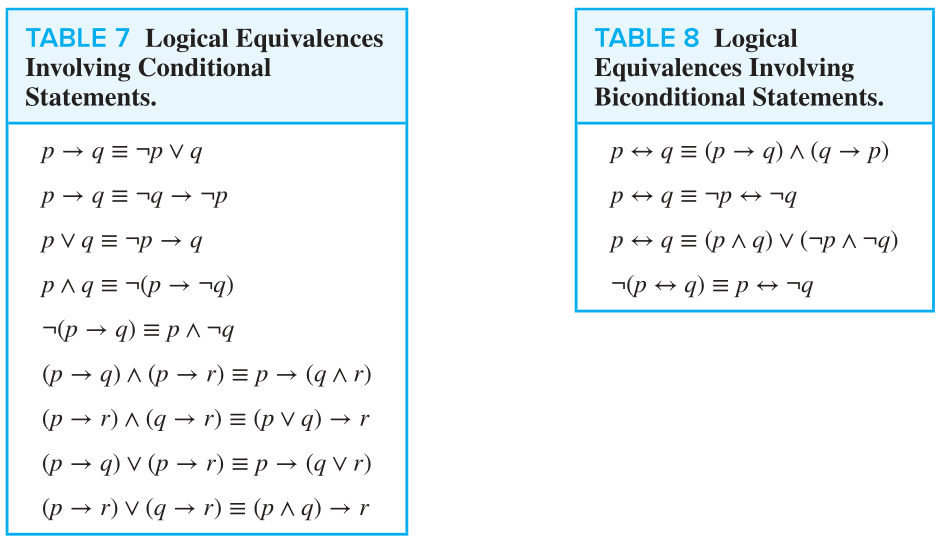
\includegraphics[width=\linewidth]{assets/equivalences.png}
						\label{uquivalences}
						\caption{Equivalences of conditional and biconditional statements}
					\end{figure}
					\subsubsection{Applying equivalences}
					By applying equvalences it is possible to show $\neg(P\lor (\neg P \land Q))\equiv \neg P \land \neg Q$\\
					\begin{align*}
						\neg(P\lor(\neg P \land Q))&\equiv \neg P\land\neg(\neg P\land Q) && \text{second De Morgan law}\\
									   &\equiv \neg p \land \neg (\neg P)\lor \neg Q && \text{first De Morgan Law}\\
									   &\equiv \neg P \land (P \land \neg Q) && \text{double negation law}\\
									   &\equiv (\neg P \land P)\lor(\neg P \lor \neg Q) && \text{second distributive law}\\
									   &\equiv F \lor (\neg P \lor \neg Q) \\
									   &\equiv \neg P \land \neg Q
					\end{align*}
					$\neg(P\rightarrow Q)\equiv \neg (\neg P\lor Q)$
					\begin{align*}
						\neg(P\rightarrow Q) &\equiv \neg (\neg P \lor Q) && P\rightarrow Q\equiv \equiv \neg P \lor Q\\
								  &\equiv\neg (\neg P) \land \neg Q) && \text{ifølge De Morgan}\\
								  &\equiv P \land \neg Q &&\neg(\neg P) \equiv P
					\end{align*}
			\subsection{Logic gates}
				The following is translations of logic operators to gates\\
				\begin{figure}[h]
					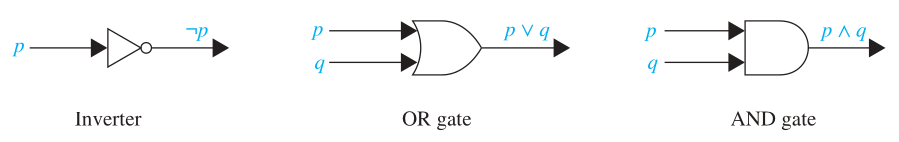
\includegraphics[width=\linewidth]{assets/gates.png}
					\label{gates}
					\caption{Gates and logical operations}
					\end{figure}
			
			\subsection{Tal grupperinger}
				$\mathbb{Z}$ heltal {...,-2,-1,0,1,2,3,...}\\
				$\mathbb{Z}^+$ Positive heltal {1,2,3,...}\\
				$\mathbb{Z}^-$ Negative heltal {-1,-2,-3,...}\\
				$\mathbb{N}$ Naturlige tal {0,1,2,3,4,...} - 0 er ikke altid inkluderet\\
				$\mathbb{Q}$ Rationale tal {$\frac{m}{n}|m\in \mathbb{Z} , n \in Z^+$}
				$\mathbb{R}$ Reelle tal
			\subsection{Kvantorer}
				Åbent udsagn - ukendt variable\\
				Har altid den højeste procedens og tages altid først.\\
				$P(x): 2x > x$\\
				Ukendt variable - fri variabel\\
				Herfra fungere det som funktion\\
				$p(-2): 2\cdot (-2)>-2$ - F\\
				$\forall$ alkvartor/universel quantifier - for alle\\
				eks.\\
				$\forall x \in \mathbb{Z}^+ : 2x > x$ - S\\
				Alle positive heltal vil være sandt.\\
				Ydelgiere notations eksempel:\\
				$\forall x \in Z: (x \leq 5 \rightarrow 2x > x +4)$\\
				$\exists$ Eksistenskvantor/Existenstial quantifier\\
				Påkræver kun at der eksistere et x i intervallet som opfylder udsagnet.\\
				$\exists x \in \mathbb{Z}, x\leq 10: Q(x)$\\
				$\exists x \in \mathbb{Z}: (x\leq 10 \land Q(x)$\\
				$\exists !$ Eksistere kun 1 variable værdi som passer, mere gør den falsk\\
				$\neg \forall x \in s: P(x)\equiv \exists x \in S : \neg P(x)$\\
				$\neg \forall x \in \mathbb{Z} : 2x>x \iff \exists x \in \mathbb{Z} : 2x \leq x$\\
				$\nexists \equiv \neg \exists$
				\subsubsection{De Morgans love for kvantorer}
					$\neg \forall x: P(x) \equiv \neg \exists x: \neg P(x)$\\
					$\neg \exists ! x : P(x) \equiv \forall x: P(x) \lor \exists x,y:(x\neq y \land P(x) \land P(y))$\\[5mm]
					Eksempel:
					\begin{align*}
						\neg \forall x \in \mathbb{Z} &:(x<4 \lor x > 4)\\
						\exists x \in \mathbb{Z} &: \neg(x<4 \lor x >4 ) && \neg\forall \equiv \exists\\
								 &: (\neg(x<4) \land \neg (x>4)) && \neg (P \lor Q)\equiv (P \land Q)\\
								 &: (x \geq 4 \land x \leq 4) && \text{negering af operator}\\
								 &: x = 4 && \text{Simplificering af udtrykket}
					\end{align*}
				\subsubsection{Indlejrede kvantorer}
					Eksempel:\\
					$\forall x \in \mathbb{Z} : \exists y \in \mathbb{Z} : x+y=0$ | Sandt $ (x=-y)$\\
					For alle x findes 1 y som vil resultere i additionen giver 0\\
					Rækkefølgen er vigtig for forskellige kvantorer, ved ens kvantorer er rækkefølgen ikke vigtig.\\
					$\forall y \in \mathbb{Z}: \forall x \in \mathbb{Z} \equiv \forall x \in \mathbb{Z}: \forall y \in \mathbb{Z}$\\
					I samme univers kan det også forkortes.\\
					$\forall x,y \in \mathbb{Z}$\\[5mm]
					Eksempel på én negering af indlejrede kvantorer\\
					\begin{align*}
						\neg\exists x \in \mathbb{Z}:\forall y \in \mathbb{Z}:x>y\\
						\forall x \in \mathbb{Z}:\neg\forall y \in \mathbb{Z}: x>y\\
						\forall x \in \mathbb{Z}:\exists y \in \mathbb{Z}: \neg(x>y)\\
						\forall x \in \mathbb{Z}:\exists y \in \mathbb{Z}: x \geq y
					\end{align*}
		\section{Bevismetoder}
			Beviser typer
			\begin{itemize}
				\item Direkte bevis - Klassisk udledningsbevis
				\item Kontra positionsbevis - Bevise det \; mod \;satte
				\item \; mod \;stidsbevise - Starte med den \; mod \;satte antagelse og finde en \; mod \;strid
			\end{itemize}
			\subsection{Direkte bevis}
				Eksemple på direkte bevis
				\begin{align}
					\text{lige tal} &= \exists k\in\mathbb{Z}: n =2k\\
					\text{ulige tal} &= \exists k \in \mathbb{Z}: n=2k+1\\[8mm]
					\exists k \in \mathbb{Z}&: n=2k+1\\
								&: n^2=4k^2+1+4k\\
								&: n^2 = 2(2k^2+2k)+1\\[4mm]
					n^2 &= \text{ulige}
				\end{align}
				Det kan konkluderes ud fra (5) at det i parentesen kan beskrive alt i domænet $\mathbb{Z}$ og dermed fåes definitionen på ulige tal. Dermed bliver det her bevist $n \text{ ulige} \rightarrow n^2 \text{ ulige}$. 
			\subsection{Kontrapositionsbevis}
			 Eksempel som efterfølger sidste bevis 
			 	For at kunen bevise at $n^2 \text{ ulige} \iff n \text{ ulige}$ skal følgende også kunne siges$n^2 \text{ ulige} \rightarrow n \text{ ulige}$
				\begin{align}
					\exists k \in \mathbb{Z}&: n=2k\\
								&:n^2=4k^2=2\cdot 2k^2\\
					n^2&=\text{lige}
				\end{align}
				Der tages her udgangspunkt i de lige tal $n$ hvorfra det kan omskrives til, at $n^2$ er lige\\
				Med dette udgangspunkt vil det betyde det kun kan passe at $n^2 \text{ ulige} \iff n \text{ ulige}$ 
			\subsection{\; mod \;stidsbevis}
				Eksempel\\
				For enhver retvinklet trekant gælder $c < a+b$\\
				Bevis: Antag til \; mod \;stad, at der ekstistere en trekant med $\geq a+b$
				\begin{align*}
					c&\geq a+b\\
					c^2&\geq (a+b)^2\\
					c^2&\geq a^2+b^2+2ab
				\end{align*}
				Det kan her ses at \; mod \;striden er forkert da den er i \; mod \;strid med Pythagoras sætning.
			\subsection{Ikke konstruktiv eksistensbevis}
				Eksempel\\
				For en funktion $f(x)=x^4-x^2-1$ vides det at når x er 0 er y -1 og ved x er 2 er y 11 og da den er kontinuer vil der være et nul punkt imellem.
			\subsection{Induktions bevis}
				Bevis $P(n)$ for alle $n\geq m$\\
				Basis: bevis $P(m)$\\
				Induktionsskridt: Bevis at $P(k)\rightarrow P(k+1)$ for alle $k\geq m$\\
				Induktionsantagelse: $P(k)$
			\subsection{Stærkt induktion}
				Basis: Bevis $P(m), P(m+1),...,P(m+l), l\geq 0$\\
				Induktionsskridt: Bevis $P(m)\land P(m+1)\land ... \land P(k)\rightarrow P(k+1)$, for alle $k\geq m+l$\\
				Eks. \\
				Bevis $f_n>\phi^{n-2},n\geq 3$\\
				\begin{align*}
					\phi^2&=(\frac{1+\sqrt{5}}{2})^2=\frac{1+5+2\sqrt{5}}{4}=\frac{3+\sqrt{5}}{2}=1+\frac{1+\sqrt{5}}{2}\\
					\phi\approx 1.618
					\phi^2&=1+\phi
					\text{Basis}\\
					f_3&=2\\
					\phi^{3-2}&=\phi<f_3\\
					f_4&=3\\
					\phi^{4-2}&=1+\phi<f_4\\[4mm]
					\text{Induktionsantagelse}\\
					f_{k-1}>\phi^{k-3}\text{og} f_k>\phi^{k-2}\\[4mm]
					\text{Induktionsskridt} k\geq 4\\
					f_{k+1}&=f_k+f_{k-1}\\
					&>\phi^{k-2}+\phi^{k-3}\\
					&=\phi^{k-5}(\phi+1)\\
					&=\phi^{k-3}\cdot \phi^2\\
					&=\phi^{k-1}
				\end{align*}
			\subsection{Strukturel induktion}
				Induktion basseret på rekursion.
				\subsubsection{Eksempel}
					Bevis for at $S_n=S_{n-1}\cup \{x+y|x,y\in S_{n-1}\}, n \geq 2$ hvor mængden er kaldet $S$ er lig med mængden $A=\{3n|n\in\mathbb{Z}^+\}$\\
					Bevis med simpel induktion at $A\subseteq S$:\\
					\begin{align*}
						\text{Basis:}& 3\cdot 1 \in S_1\ \subseteq S
						\text{Ind. ant:}&\;3k\in s, \text{for et }\; k\geq 1\\
						\text{Ind. skridt: For}&\; k\geq 1 \; \text{gælder}\\
						3(k+1)&=3k+3 &&\text{begge i S}\\
						3(k+1)&\in S &&\text{Ifølge rek. skridt}
					\end{align*}
					Dermed er alle multiple i $S$ dermed skal det blot vises at $S\subseteq A$ med strukturel induktion.
					\begin{align*}
						\text{Basis:}& S_1 \subseteq A\\
						\text{Ind. ant:}&\;S_k\subseteq A\\
						\text{Ind. skridt: For}&\; S_k \subseteq A \rightarrow S_{k+1}\subseteq A:\\
						S&\in S_{k+1}-S_k\\
						S&=x+y, x,y\in S_k && \text{ifølge rek. skridt}\\
						S&=3a+3b, a,b\in \mathbb{Z}^+&&\text{ifølge ind. ant.}\\
						S=3(a+b), a+b\in\mathbb{Z}^+\\
						S\in A
					\end{align*}
		\section{Mængder} 
			En mængde/set er en uordnet samling af forskellige objekter kaldet elementer\\
			\begin{align*}
				A&=\{1,2,3\}=\{3,1,2\}=\{3,1,1,2,3\}\\
				2&\in A - True\\
				B&=\{1,\{2,4\},a\}\\
				\{2,4\}&\in B - True\\[5mm]
				\mathbb{N}&=\{0,1,2,...\}\\
				\mathbb{Z}&=\{...,-2,-1,0,1,2,...\}
			\end{align*}
			\subsection{Mængde-bygger-notation}
				\begin{align*}
					L&=\{0,2,4,6,...\}\\
					 &=\{2n|n\in\mathbb{N}\}\\
					 &=\{n|\exists k \in \mathbb{N}:n=2k\}\\
					 &=\{n\in\mathbb{N}| n/2\in\mathbb{N}\}
				\end{align*}
				$|$ = "hvorom der gælder"\\
				$\emptyset = \{\}$\\
			\subsection{Kardinalitet}
				Kardinaliteten er mængden af unikke elementer i en liste\\
				$|\{2,2,4,6,4\}|=3$\\
				Delmængde $A\subset B$ $A=\{1,2\}$ $B=\{1,2,3,4\}$\\
				$\subseteq$ bruges hvis mængderne også må være lig hinanden. En ægte delmængde er en delmængde som ikke er lig med.\\
				$\subset \iff A\subseteq B \land A\neq B$
				\begin{align*}
					\emptyset \subseteq A\\
					\forall x \in \emptyset : x \in A\\
					\forall x \in U : x\in \emptyset \rightarrow x \in A
				\end{align*}
			\subsection{Potensmængde}
				Potensmængden er alle mængder som er delmængder eller lig med mængden.\\
				\begin{align*}
					C=\{1,2\}\\
					P(C)=\{\emptyset,\{1\},\{2\},\{1,2\}
				\end{align*}
				Potenslængden på mængden med $i$ elementer vil være $2^i$
			\subsection{Karteisisk produkt}
				To mængders kartesiske produkt er en mængde bestående af 2 elementer fra hver mængde. Længden på 2 elementer kaldes også 2-tupler\\
				\begin{align*}
					A=\{1,2\}, B=\{2,3\}\\
					A\times B = \{(1,2),(1,3),(2,2),(2,3)\}\\
					|A\times B| = |A| \cdot |B|
				\end{align*}
				Kardinaliteten af et kartesisk produkt er kardinaliteten af de to mængder multipliceret sammen.\\
			\subsection{Intervaller}
				\begin{align}
					[a,b]=\{x\in \mathbb{R}| a\leq x \leq b \}\\
					]a,b[/(a,b) = \{x\in \mathbb{R} | a< x < b\}\\
					[a,b)=\{x\in \mathbb{R} | a \leq x < b\}\\
					(a,b] = \{x\in \mathbb{R} |a < x \leq b\}
				\end{align}
				\begin{enumerate}
					\item Lukket mængde
					\item Åben mængde
					\item Halvåben mængde
					\item Halvåben mængde
				\end{enumerate}
			\begin{align*}
				A=\{1,2,3\}\\
				B=\{2,3,4\}\\
				U=\mathbb{Z}
			\end{align*}
			\subsection{Foreningsmængde}
				
				\begin{minipage}{0.45\textwidth}
				$A\cup B = \{x|x\in A \lor x \in B\}$\\
				$A\cup B = \{1,2,3,4\}$\\[3mm]
				$A\cup B = \;\text{Det hele blå felt} $
				\end{minipage}
				\hfill
				\begin{minipage}{0.45\textwidth}
				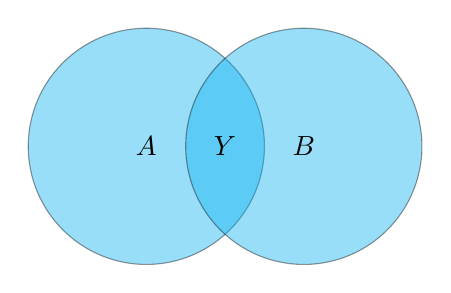
\begin{tikzpicture} [set/.style = {draw,
					    circle,
					    minimum size = 3cm,
					    fill=cyan,
					    opacity = 0.4,
					    text opacity = 1}]
					 
					\node (A) [set] {$A$};
					\node (C) at (0:2cm) [set] {$B$};
					\node at (barycentric cs:A=1,C=1)  {$Y$};
				\end{tikzpicture}
				\end{minipage}
			\subsection{Fællesmængde}
				\begin{minipage}{0.45\textwidth}
				$A\cap B =\{x| x\ in A \land x \in B \}$\\
				$A\cap B = \{2,3\}$\\
				$A\cap B = \;\text{Y} $
				\end{minipage}
				\hfill
				\begin{minipage}{0.45\textwidth}
				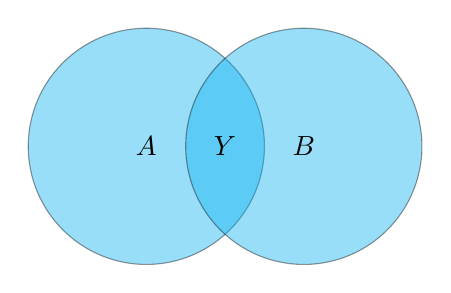
\begin{tikzpicture} [set/.style = {draw,
					    circle,
					    minimum size = 3cm,
					    fill=cyan,
					    opacity = 0.4,
					    text opacity = 1}]
					 
					\node (A) [set] {$A$};
					\node (C) at (0:2cm) [set] {$B$};
					\node at (barycentric cs:A=1,C=1)  {$Y$};
				\end{tikzpicture}
				\end{minipage}
			\subsection{Fraregnet}
				\begin{minipage}{0.45\textwidth}
				$A\setminus B \equiv A-B$\\
				$A\setminus B = \{x | x \in A \lor \notin B\}$\\
				$A\setminus B = \{1\}$\\
				$A\setminus B = \;\text{Kun helt røde} $
				\end{minipage}
				\hfill
				\begin{minipage}{0.45\textwidth}
				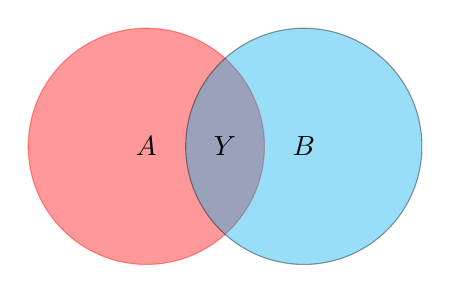
\begin{tikzpicture} [set/.style = {draw,
					    circle,
					    minimum size = 3cm,
					    fill=cyan,
					    opacity = 0.4,
					    text opacity = 1}]
					 
					\node (A) [set,color=red] {$\color{black}A$};
					\node (C) at (0:2cm) [set] {$B$};
					\node at (barycentric cs:A=1,C=1)  {$Y$};
				\end{tikzpicture}
				\end{minipage}
			\subsection{Komplementet}
				$\overline{A} = u-A$
			\subsection{Disjunkte}
				To mængder er disjunkte hvis 
				\begin{align*}
					A\cup  B = \emptyset\\
					\neg \exists x: x \in \land x \in B\\
					A\subseteq \bar{B}\\
					B\\ A = B
				\end{align*}
			\subsection{Mængde love}
				For at overbevise sig selv om love kan venn diagramer bruges som sandhedtabeller kunne bruges tidligere.
				\begin{center}
					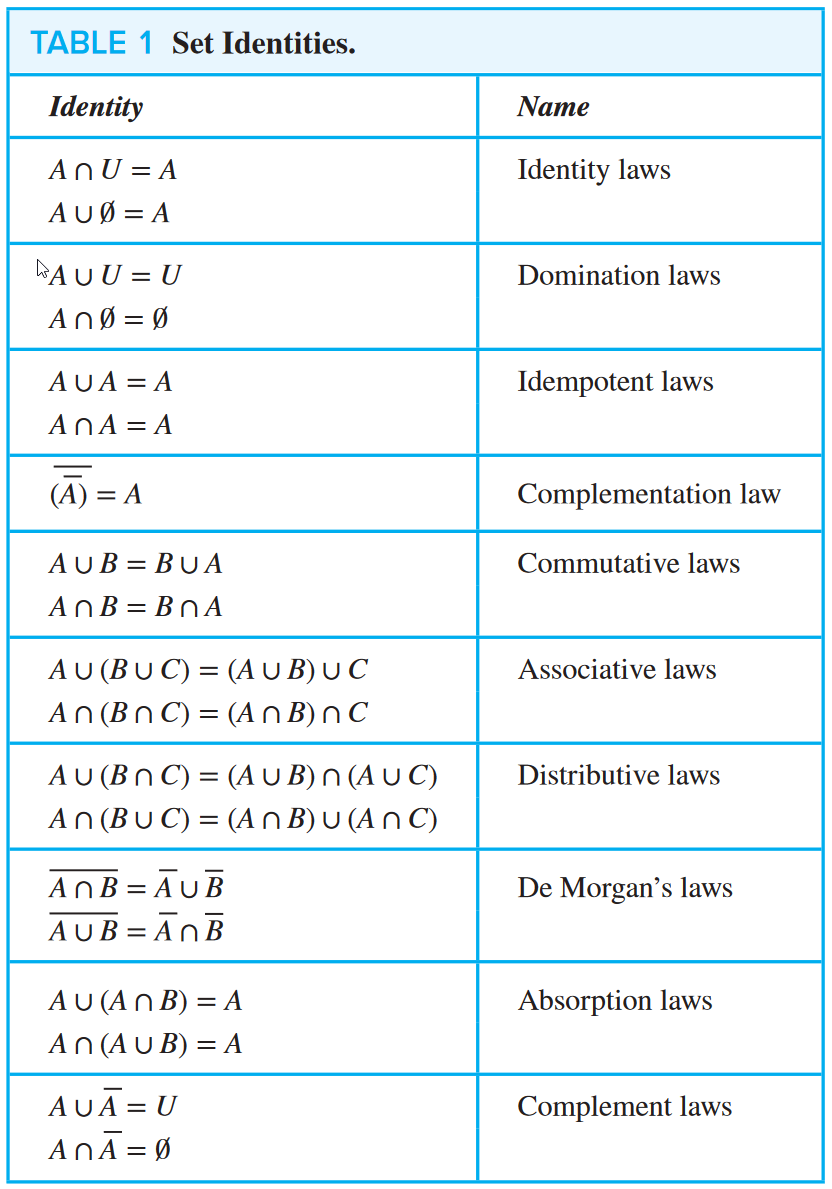
\includegraphics[width=300px]{assets/setEq.png}
				\end{center}
				\subsubsection{De Morgans love}
					$\overline{A\cap B} = \overline{A}\cup \overline{B}=u-(A\cap B)$\\
					$\overline{A\cup B} = \overline{A} \cap \overline{B}$\
			\subsection{Ydeligere notation}
				\begin{align*}
					\bigcup\limits_{i=1}^n A_i=A_1\cup A_2 \cup ... \cup A_n\\
					\bigcap\limits_{i=1}^n A_i=A_1\cap A_2 \cap ... \cap A_n
				\end{align*}
				Alfabet - mulige tegn i en mængde eks. $\Sigma = \{0,1\}$ for bit strings\\
				Yderligere gælder det $\Sigma^*$ ligesom i regulære udtryk er en samling af tegn i alfabettet, hvor der er 0 eller flere tegn.
			\section{Funktion}
				En funktion er en translation af elementer fra en definitionsmængde, hvor hvert element i A har en tilsvarende element i B.\\
				Defintionsmængde $Dm(f)$\\
				Værdimængde 
				\begin{align*}
					Vm(f)&={y\in B \ \exists x \in A: f(x)=y}\\
						&={f(x)|x\in A}\\
						&=f(A)
				\end{align*}
				\subsection{Injektive funktioner}
					$\forall x_1,x_2 \in Dm(f): f(x_1)=f(x_2)\rightarrow x_1=x_2$\\
					Alle x værdier vil have sin egen y værdi.
				\subsection{Surjektiv}
					$\forall y \in B: \exists x \in A: f(x)=y$\\
					Der findes en x i definitionsmængden så alle værdimængder / y værdier bliver ramt.
				\subsection{Bijektiv}
					Funktionen er både injektiv og surjektiv\\
					Alle punkter i y bliver ramt én gang. 1 til 1 korrestance 
				\subsection{Invers funktion}
					Isolering af x.\\
					Ved afbilledring vil akserne byttes rundt\\
					Ikke det samme som $f^{-1}$ som er bare $\frac{1}{f(x)}$\\
					Ved afbilledring vil akserne byttes rundt
				\subsection{Operationer på funktioner}
					Her vil blot de funtkioerne indsættes med parentes rundt om og udregnes.
				\subsection{Sammensat funktion}
					Bruger 1 funktion som værdi til funktionen.\\
					$(g\cdot f)(x)=g(f(x))$
				\subsection{Monotoniforhold}
					Strengt voksende, påkræver det at hvis $x$ er større end tidligere skal $y$ være større.\\
					Voksende kan næste $x$ værdi og være lig med $y$.\\
					Monoton - voksende eller aftagende.
				\subsection{Tællelige mængder}
					Mængden $\mathbb{Z}$ er en tællelig mængde og beskrives ved $\aleph_0$.\\
					Ikke tællelige mængder kaldes overtællige mængder.\\
					Kardinaliteten kan her bruges så hvis $\mathbb{Z}$ kan mappes til en ny mængde er den tællelig.\\
					Mængden $Q = {\frac{p}{q}|p,q\in \mathbb{Z}}$ er en tællelig mængde.\\
					Da der blot mappes en sammenhæng hvor alle $\mathbb{Z}$ kan mappes på tæller og nævner, således alle rationelle tal kan opstå og dermed er $\aleph_0$.
				\subsection{Overtællelige mængder}
					Realle tal $\mathbb{R}$ er en overtællelig mængde og kan vises via argumentet. At selv ved delmængden mellem 0 og 1 vil et nyt decimal altid kunne findes ved at age diagonalen af allerede nævnte realle tal.
			\section{Relationer}
				Relationer bruges til at finde elementer som opfylder en relation i mængder.\\
				Der er to typer af relationer kvartær og binære relationer. Binær er når der er en direkte relation, hvor kvartær har interne relationer.\\
				Eks. 
				\begin{align*}
					R_{inv}&=\{(a,b)\in \mathbb{Z}^+\times\mathbb{R}^+|b=\frac{1}{a}\}\\
					&=\{(1,1),(2,\frac{1}{2}),(3,\frac{1}{3}),...\}\\
					(2,\frac{1}{2})&\in R_{inv}\\
					(\frac{1}{2},2)&\notin R_{inv}\\
					5R_{inv}\frac{1}{5}
				\end{align*}
				En relation på mængden $A$  er en relation fra $A$ til $A$, dvs $(a,b)\in A\times A|...$
				\subsection{Matriar}
					Her bruges en matrix med række og collonner som repræsentere de forskellige elementer hvor 0 er falsk og 1 er sandt.\\
					\begin{align*}
					A=\{1,2,3\} - R_<&=\{(a,b)\in A\times A | a<b\} = \{(1,2),(1,3),(2,3)\}\\
					\begin{bmatrix}
					0 & 1 & 1\\
					0 & 0 & 1\\
					0 & 0 & 0
					\end{bmatrix}
					\end{align*}
				\subsection{Orienterede grafer}
				\begin{minipage}{0.75\textwidth}
						Her bruges en graf, hvor relationer er repræsenteret som en kant og hvert element er en knude.\\
						$A=\{1,2,3,4\} - R_p$\\
						$=\{(a,b) | a $ og $b$ har samme paritet$\}$ \\
						$= \{(1,1),(1,3),(2,2),...\}$\\
					\end{minipage}
					\hfill
				\begin{minipage}{0.15\textwidth}
					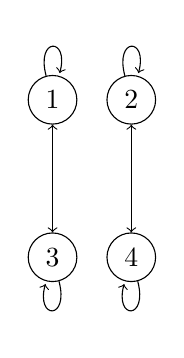
\begin{tikzpicture}[scale=1]
						\tikzstyle{vertex}=[circle,draw=black]
						\node[vertex](v1) at (0,2) {1};
						\node[vertex](v2) at (1,2) {2};
						\node[vertex](v3) at (0,0) {3};
						\node[vertex](v4) at (1,0) {4};
						\path(v1) edge [loop above] node {}(v1);
						\draw[<->](v1) -- (v3);
						\path(v3) edge [loop below] node {}(v3);
						\path(v2) edge [loop above] node {}(v2);
						\draw[<->](v2) -- (v4);
						\path(v4) edge [loop below] node {}(v4);
					\end{tikzpicture}
					\end{minipage}
				\subsection{Egenskaber}
					\subsubsection{Refleksiv}
						Mængden $R$ relation på $A$ er kun refleksiv hvis $$(a,a)\in R$$, for alle $a\in A$\\
						$\{(1,1),(2,2),(3,3)\}$ på $\{1,2,3\}$ er sand\\
						$\{(1,1),(2,2)\}$ på $\{1,2,3\}$ er falsk\\
						Følgende diagonal skal være sand hele vejen for refleksiv i en matrise. Et diagram påkræver alle knuder har en lykke til sig selv.\\
						\begin{align*}
						\begin{bmatrix}
						1 & 0 & 0\\
						0 & 1 & 0\\
						0 & 0 & 1
						\end{bmatrix}				
						\end{align*}
					\subsubsection{Symmetrisk}
						Mængden $R$ relation på $A$ er kun symmetrisk hvis $$(a,b)\in R \rightarrow (b,a)\in R$$, for alle $a,b\in A$\\	
						$\{(1,3),(3,1)\}$ og $=$ sand\\
						$>$ falsk\\
						På et diagram skal alle kanter vende begge retninger. På en matrise kan det genkendes ved at der skal være en spejling på diagonalen således:\\
						\begin{align*}
						\begin{bmatrix}
						\smallsetminus    & 0 & 0\\
						0 & \smallsetminus & 0\\
						0 & 0 & \smallsetminus
						\end{bmatrix}			
						\end{align*}
					\subsubsection{Anti-symmetrisk}
						Mængden $R$ relation på $A$ er kun anti-symmetrisk hvis $$(a,b)\in R\land (b,a)\in R \rightarrow b=a$$, for alle $a,b\in A$\\	
						$< \& =$ sand\\
						$\neq$ falsk\\
						På en matrise må der ikke være en spejling på aksen.
						\begin{align*}
						\begin{bmatrix}
						\smallsetminus    & 0 & 0\\
						0 & \smallsetminus & 0\\
						0 & 0 & \smallsetminus
						\end{bmatrix}			
						\end{align*}
					\subsubsection{Transitiv}
						Mængden $R$ relation på $A$ ertransitiv hvis $$(a,b)\in R\land (b,c)\in R \rightarrow(a,c)\in R$$, for alle $a,b,c\in A$\\	
						$\{(1,2),(1,3),(1,4),(2,3),(2,4),(3,4)\}$ og $<$ sand\\
						$\{(1,2),(1,3),(2,3),(3,4)\}$ og $\neq$ falsk\\
						På et diagram er det nemt at se om der mangler direkte kanter efter to kanter.
			\subsection{Kombination af relationer}
				Mængde operationer kan udføres på relationer.\\
				Herudover kan sammensættes osm funktioner.\\
				\begin{align*}
					R: \; \text{relation fra}\; A \;\text{til}\; B\\
					S: \; \text{relation fra}\; B \;\text{til}\; C\\
					S\circ R=\{(a,c)|\exists b: (a,b)\in R\land (b,c)\in S\}
				\end{align*}\\[5mm]
				\begin{minipage}{0.45\textwidth}
				$\color{blue}R\color{black}=\{(1,2),(3,1)\}$\\
				$\color{red}S\color{black}=\{(1,3),(2,2),(2,3)\}$\\
				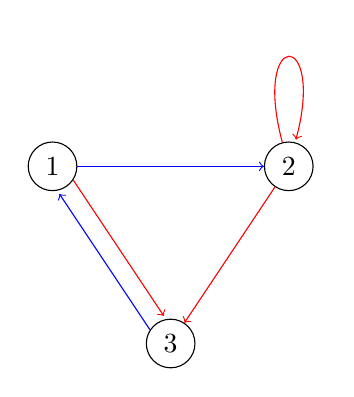
\begin{tikzpicture}[scale=3]
						\tikzstyle{vertex}=[circle,draw=black]
						\node[vertex](v1) at (0,0.75) {1};
						\node[vertex](v2) at (1,0.75) {2};
						\node[vertex](v3) at (0.5,0) {3};
						\draw[red, ->,transform canvas={xshift=2.5pt,yshift=2.5pt}](v1) -- (v3);
						\draw[blue, <-,transform canvas={xshift=-2.5pt,yshift=-2.5pt}](v1) -- (v3);
						\draw[blue,->](v1) -- (v2);
						\draw[red,->](v2) -- (v3);
						\path(v2) edge [loop above, color=red] node {}(v2);
					\end{tikzpicture}
				\end{minipage}
				\hfill
				\begin{minipage}{0.45\textwidth}
				$\color{cyan}S\circ R\color{black}=\{(1,1),(2,1)\}$\\\
				$\color{purple}R\circ S\color{black}=\{(1,2),(1,3),(3,3)\}$\\
				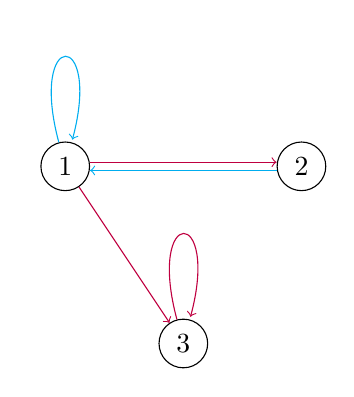
\begin{tikzpicture}[scale=3]
						\tikzstyle{vertex}=[circle,draw=black]
						\node[vertex](v1) at (0,0.75) {1};
						\node[vertex](v2) at (1,0.75) {2};
						\node[vertex](v3) at (0.5,0) {3};
						\draw[purple,->,transform canvas={yshift=1.5pt}](v1) -- (v2);
						\draw[purple,->](v1) -- (v3);
						\draw[cyan,->,transform canvas={yshift=-1.5pt}](v2) -- (v1);
						\path(v3) edge [loop above, color=purple] node {}(v3);
						\path(v1) edge [loop above, color=cyan] node {}(v1);
					\end{tikzpicture}
				\end{minipage}\\[3mm]	
				\begin{center}
					Sammensat kan findes ved at følge den første relations kanter efterfulgt af den andens relations kanter.
				\end{center}
			\subsection{Lukninger }
				Lukninger bruges til at gøre relationer for en given egenskab.\\
				Følgende former for lukning vil eksemplerne tage udgangspunkt i $$R=\{(1,3),(2,2),(2,3,(3,1),(3,3)\}$$

				\subsection{Refleksive lukninger}
					Eksempelvis. Den refleksive lukning af $R$ er $r(R)=R\cup \{(a,a)|a\in A\}$\\
					$r(R)=R\cup \{(1,1),(4,4)\}$\\
					Eksempel på en uendelig tællelig mængde:\\
					$R_<=\{(a,b)|a<b\}$\\
					$r(R_<)=R\cup \{(a,b)|a=b\}$
				\subsection{Symmetriske lukninger}
					$R$ er en relation på $A$ gælder det at den symmetriske lukning er:\\
					$s(R)=R\cup\{(a,b)\in A\times A|(b,a)\in R\}$\\
					$S(R_<)=R_< \cup R_> = R_{\neq}$\\
					$(s(R)=R\cup \{(3,2)\}$
				\subsection{Transivativ lukning}
					Den transative lukning vil indeholde kan defineres ved \\
					$t(R)=R^*=\bigcup\limits_{i=1}^{|A|} R^i$ Hvis $A$ er endelig\\
					her tages fællesmængden af relationen og relationen sammensat med sig selv og relationen sammensmat med sig selv 3 gange osv.\\
					$t(R)=R\cup \{(2,1)\}$
			\section{Ækvivalensrelationer}
				En ækvivalensrelation er reflekstiv, symmetrisk og transitiv.\\
				Eks. parietet, = og den tomme relation er en ækvivalens\\
				$a$ og $b$ som tilhøre en ækvivalens relation er ækvivalente\\
				\textbf{Ækvivalensklassen} for $a$ er $[a]_R=\{b|(a.b)\in R\}$ D.V.S alle elementer som er relateret til $a$ for $R$ som er en ækvivalens relation på $A$\\ 
				En relation ækvivalensklasser vil altid være dækket af hele relationen også kaldet \textbf{partitionær}.\\
				\subsection{Partitionær}
					For den ækvivalente relation da gælder: \\
					\begin{itemize}
						\item $a R b$
						\item $[a]_R=[b]_R$
						\item $[a]_R\cap [b]_R\neq \emptyset$
					\end{itemize}
					D.V.S to relateret elementer, må være i samme ækvivalens klasse og de to klassers overlap ikke må være tomt.\\
					Det vil her bevises at $(1)\rightarrow (2)\rightarrow (3)\rightarrow (1)$ dermed alle 3 udtryk er ækvivalente.
					\subsubsection{$a R b\rightarrow [a]_R=[b]_R$}
						Et \; mod \;stridsbevis kan her opstilles.\\
						Et punkt som er relateret til $a$ og ikke er relateret til $b$ er ikke mulig, da $R$ ikke længere vil være transitativ.
					\subsubsection{$[a]_R=[b]_R\rightarrow [a]_R\cap [b]_R\neq \emptyset$}
						Den eneste måde hvorpå at overlappet kan være tomt påkræver at $[a]_R=\emptyset$\\
						Dette kan dog ikke lade sig gøre, da $a$ er en del af sættet og pr. definition er ækvivalensklassen reflektiv og dermed er elementet $(a,a)$ altid i $[a]_R$.
					\subsubsection{$[a]_R \cap [b]_R \neq \emptyset \rightarrow a R b$}
						Efter at overlappet ikke er tomt, vil det betyde der et et punkt $c$ som er relativ til $a$ og $b$. Dermed da ækvivalensklassen er transitativ vil det medføre at $a$ er relateret til $b$\\[5mm]
					\subsection{Ækvivlanesklasserne dækker hele $A$}
						Dette ville påkræve at to ækvivalensklasser ikke overlapper hinanden.\\
						For ækvivalens klassen vides det at $\forall a \in A: a\in [a]$\\
						Dermed vides det at klassen ikke er tom og da for to klasse som er ens $[a]\cap [b]\neq \emptyset$ \\
						Det kan så vendes rundt (negeres) at hvis deres overlap er tomt $[a]\cap [b]=\emptyset$ vil det medføre $\neg([a]=[b])$ altså $[a]\neq [b]$.\\
						Dermed kan to ækvivalensklasser ikke overlappe.
									
			\section{Partiel ordning}
				Relfleksive, transitive og antisymetrisk.\\
				\textbf{Partielt ordnet mænde} $(A,R)$ hvor $R$ er en mængde på $A$ som er en partiel ordning.\\
				Eks. = og $\geq$\\
				$(\{1,2,3,4,5,6,7,8\},|)$ hvor $|$ er går op i.\\
				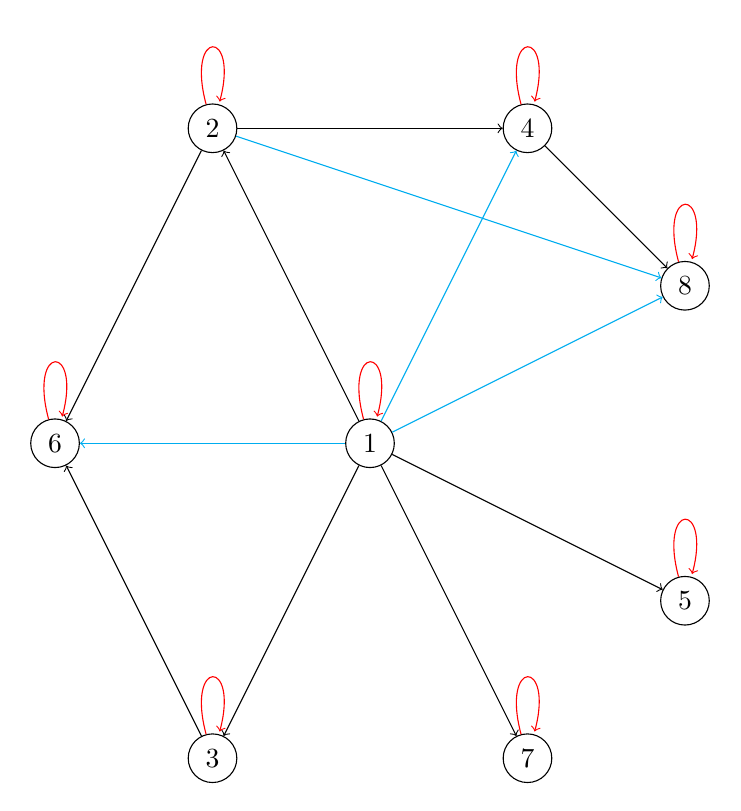
\begin{tikzpicture}[scale=2]
						\tikzstyle{vertex}=[circle,draw=black]
						\node[vertex](v1) at (2,2) {1};
						\node[vertex](v2) at (1,4) {2};
						\node[vertex](v3) at (1,0) {3};
						\node[vertex](v4) at (3,4) {4};
						\node[vertex](v5) at (4,1) {5};
						\node[vertex](v6) at (0,2) {6};
						\node[vertex](v7) at (3,0) {7};
						\node[vertex](v8) at (4,3) {8};
						\draw[cyan,->](v1) -- (v6);
						\draw[cyan,->](v1) -- (v4);
						\draw[cyan,->](v1) -- (v8);
						\draw[cyan,->](v2) -- (v8);
						\draw[black,->](v1) -- (v5);
						\draw[black,->](v1) -- (v7);
						\draw[black,->](v1) -- (v3);
						\draw[black,->](v1) -- (v2);
						\draw[black,->](v3) -- (v6);
						\draw[black,->](v2) -- (v6);
						\draw[black,->](v2) -- (v4);
						\draw[black,->](v4) -- (v8);

						\path(v1) edge [loop above, color=red] node {}(v1);
						\path(v2) edge [loop above, color=red] node {}(v2);
						\path(v3) edge [loop above, color=red] node {}(v3);
						\path(v4) edge [loop above, color=red] node {}(v4);
						\path(v5) edge [loop above, color=red] node {}(v5);
						\path(v6) edge [loop above, color=red] node {}(v6);
						\path(v7) edge [loop above, color=red] node {}(v7);
						\path(v8) edge [loop above, color=red] node {}(v8);
					\end{tikzpicture}
				
				\subsection{Hassediagrammer}
				Med underforståelsen at det er en partiel ordning er det ikke nødvendigt at vise alle direkte kanter\\
				\begin{tikzpicture}[scale=2]
						\tikzstyle{vertex}=[circle,draw=black]
						\node[vertex](v1) at (2,0) {1};
						\node[vertex](v2) at (1,1) {2};
						\node[vertex](v3) at (0,1) {3};
						\node[vertex](v4) at (2,2) {4};
						\node[vertex](v5) at (3,1) {5};
						\node[vertex](v6) at (1,2) {6};
						\node[vertex](v7) at (4,1) {7};
						\node[vertex](v8) at (2,3) {8};
						\draw[-](v1) -- (v3);
						\draw[-](v1) -- (v2);
						\draw[-](v1) -- (v5);
						\draw[-](v1) -- (v7);
						\draw[-](v3) -- (v6);
						\draw[-](v2) -- (v6);
						\draw[-](v2) -- (v4);
						\draw[-](v4) -- (v8);
					\end{tikzpicture}\\
					Maskimale elementer er elementer som ikke har nogle elementer relateret over sig. $\nexists b\in A: b<a$\\
					Minimlae elmenter er elementer som ikke har nogle andre lementer som går op i det.$\forall b \in A: a<b$\\
					Er det kun 1 element som er maksimal eller minimal er det den største ($\forall v \in A: b<a$) eller mindste ($\nexists b \in A: a<b$).\\
					
				\subsection{Total ordning}
					Den partielle ordning for $R$ er hvor $a R b$ eller $b R a$ er gædende. Her vil $a$ og $b$ være sammenlignelige.\\
					Er alle  par $a,b \in A$ er sammenlignelige med releationen $R$ er det en total ordning.
					Eks. \\
					$R=\{(a,b)|a\leq b\}$ på $\{1,2,3,4,5\}$ er en total ordning\\
				\subsection{Leksikografisk ordning}
					En måde hvorpå en sortering kan foregå.\\
					$(a_1,a_2)<(b_1,b_2)$\\
					Først tjekkes om $a_1<b_1$ i det tilfæde står det i leksikofrafisk ordning\\
					Hvis $a_1=b_1$ så er den leksikografisk hvis $a_2<b_2$
				\subsection{Binært træ}
					Et binært træ er et træ hvorledes hvert udkom opdeles i to muligheder. Et fuldt binært træ skal altid have to muligheder.\\
					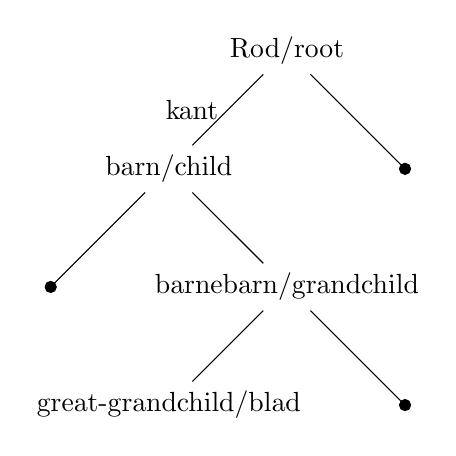
\begin{tikzpicture}
						[
						   style = {sibling distance = 3cm},
						]
						\node {Rod/root}
							child {node {barn/child}
								child {[fill] circle (2pt)}
								child {node {barnebarn/grandchild}
									child {node {great-grandchild/blad}}
									child {[fill] circle (2pt)}
								}
							edge from parent node [left] {kant}
							}
							child {[fill] circle (2pt)};
					\end{tikzpicture}\\
					De sorte punkter er kaldet knuder.\\
					For et binært træ er højden definered rekursivt således: \\$h(\circ )=0$, $h($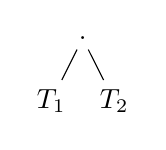
\begin{tikzpicture}
						[
						   style = {sibling distance = 0.8cm,level distance = 0.8cm}
						]
						\node {.}
							child {node {$T_1$}}
							child {node {$T_2$}};
					\end{tikzpicture}$)=max\{h(T_1),h(T_2)\}$\\
					\subsubsection{Bevis for højde på binært træ}
						$n$ antal knuder, $h$ højden og $T$ træ
						\begin{align*}
							\text{Basis:}\;& S_1=\{\circ\} = 2^{h+1}-1=1=n\\
							\text{Ind. ant:}&\;n(T)=2^{h(T)+1}-1, &&\text{for alle $T\in S_{k-1}$ $(k\geq2)$}\\
							\text{Ind. skridt:}&\; T\in S_k-S_{k-1}, &&\text{hvor}\; k\geq 2\\[4mm]
							n(T)&=1+n(T_1)+n(T_2)\\
							&\leq 1 + (2^{h(T_1)+1}-1)+(2^{h(T_2)+1}-1)&&\text{da induktions ant.}\\
							&=2^{h(T_1)+1}+2^{h(T_2)+1}-1\\
							&\leq 2^{h(T)}+2^{h(T)}-1 &&\text{da}\; h(T_1)\leq h(T) \geq h(T_2)\\
							&=2^{h(T)+1}-1
						\end{align*}
		\section{Tal teori}
			\subsection{Delelighed}
				Heltals devision kaldes $a\; div\; b$, ved negativ div rundes ned, da rest altid  skal være mellem 0 og divisor.\\
				For $a|b$ er udsagnet korrekt hvis $\frac{b}{a}\in\mathbb{Z}$\\
				For dette kan det obseveres at 
				\begin{itemize}
					\item $a|b \land a|c \rightarrow a|(b+c)$
					\item $a|b\rightarrow \forall k \in \mathbb{Z} : a|k\cdot b$
					\item $a|b\land b|c \rightarrow a|c$
					\item $A|b\land a|c \rightarrow \forall m,n \in \mathbb{Z}: a|(mb+nc)$
				\end{itemize}
				\subsubsection{Bevis $a|b\land a|c \iff a|(b+c)$}
					\begin{align*}
						&a|b\land a|c\\
						b&=k\cdot a \land c=l\cdot a,&&k,l\in\mathbb{Z}\\
						b+c&=k\cdot a + l\cdot a = (k+l)a, && k+l\in \mathbb{Z}\\
						&a|(b+c)
					\end{align*}
				Division kan udføres hvis $a|bc \land gcd(a,b)=1 \rightarrow a|c$\\
				\subsubsection{Bevis for division i af delelighed}
					\begin{align*}
						a|bc \land gcd(a,b)=1\\
						\exists s,t \in \mathbb{Z}&: sa+tb=gcd(a,b)\\
									  &: sa+tb=1\\
									  &: sac+tbc=c\\
									  &: sac=c-tbc
					\end{align*}
					Dermed da $b$ er delelig med $a$ vil det betyde for at venstre side kan være et multiplum af $a$ skal $c$ være delelig med $a$. 
				
			\subsection{Kongruence}
				To kongruente tal skrives som $a\equiv b (\; \; mod \; \; m)$ dvs. $m|(a-b)$\\
				\subsubsection{$\exists k \in \mathbb{Z}: a=b+km \iff a\equiv b (\; mod \; m)$} 
					\begin{align*}
						m|(a-b)\\
						a-b=km, &k\in\mathbb{Z}\\
						a=b+km
					\end{align*}
				Den muligmængde af $a \; mod \; m$ vil være $\mathbb{Z}_m = {0,1,2,... m-1}$\\
				Dermed kan der udføres addition og multiplikation på begge sider af $\equiv$ hvis den er sand, herudover kan der mod'en ligges til og fra på en side.\\
				Her gælder det også at hvis $c\equiv d$ vil $a+c\equiv b+d$ og $a\cdot c \equiv b\cdot d$\\
				Ved $(a+b) \; mod \; m$ eller $(a\cdot b) \; mod \; m$ kan modolo udføres ind i parentesen hvorefter operationen kan foregå.\\
				\subsubsection{Bevis for modolo ind i parentes}
					\begin{align*}
						a\equiv a \; mod \; m (\; mod \; m)\\
						b \equiv b \; mod \; m (\; mod \; m)\\
						a+b\equiv (a \; mod \; m) + (b \; mod \; m) (\; mod \; m)\\
						(a+b) \; mod \; m = ((a \; mod \; m) + (b \; mod \; m)) \; mod \; m\\[4mm]
						ab\equiv (a \; mod \; m)(b \; mod \; m) (\; mod \; m)\\
						ab \; mod \; m = ((a \; mod \; m )(b \; mod \; m)) \; mod \; m
					\end{align*}
				Division kan foregå ved $ac\equiv ab (mod m)\rightarrow a\equiv b$ hvis $gcd(c,m)=1$\\
				\subsubsection{Bevis for division ved kongruencer}
					\begin{align*}
						ac&\equiv bc (\;mod\; m)\\
						m&|(bc-ac)\\
						m&|(b-a)c\\
						m&|(b-a) &&\text{Da gcd(c,m)=1}\\
						a&\equiv b (mod\; m)
					\end{align*}
			\subsection{Linære kongruenser}
				Ligninger som indebære kongruenser fremfor ligheder. $ax\equiv b (mod\; m)$\\
				Eks. $4x\equiv 5 (mod\; 11)$, her er en løsning $x=4$\\
				Det ses at løsningerne vil have differensen $m$.
				En ligning har altid en løsning hvis $gcd(a,m)=1$, og nogle gange hvis ikke det er opfyldt.\\
				For isolering af $x$ kan den inverse til $a$ modulo $m$ bliver multipliceret på begge sider.\\
				Den inverse er fundet ved $a\cdot \bar{a}\;(mod\;m)=1$. Eks. $3\cdot x)\;(mod\;11)$ Vil $x=4$\\
				Dermed vil det kun være én multiplikativ invers hvis $gcd(a,m)=1$, dog er der stadig mulighed for løsninger\\
				Euklids algoritmen kan her bruges til at finde multiplikative invers.\\
				
			\subsection{Primtal}
				$p\in mathbb{Z}^+-{1}$ hvis $\forall a|p | a\in \mathbb{Z} = {1,p}$ er $p$ et primtal. Ellers er det sammensat.\\
				Et hvert tal $n\geq 2$ har en måde hvor det er produktet af primtal, kaldet primtals faktore\\
			\subsubsection{greatest common divider}
				def. $gcd(a,b)=max\{d| d|a \land d|b\}$\\
				Det kan også ses at $gcd$ af et tal er produktet af de primtals faktore de har tilfældes
				Hvis $gcd(a,b)=1$ er $a$ og $b$ indbyrdes primiske (relatively prime).
			\subsubsection{Least common multiplum}
				def. $lcm(a,b)=min\{m| a|m \land b|m\}$\\
				Kan også findes ved at tage primfaktorne og multiplicere sammen. Ved ens primfaktore tages mængden med højst ekspnent.\\
				Dermed $lcm(a,b)=\frac{a\cdot b}{gcd(a,b)}$
		\subsection{Euklids Algoritme}
			For $a=bq+r \rightarrow gcd(a,b)=gcd(b,r)$\\
			Eksempel på brug:
			\begin{align*}
				gcd(287,91)\\
				287=91\cdot 3 + 14\\
				91=14\cdot 6 + 7\\
				14=7\cdot 2
			\end{align*}
			Dermed er $gcd(287,91)=7$ da det er den sidste rest før 0.
			\subsubsection{Bevis}
				For dette skal følgende bevises $d|a\land d|b \iff d|b\land d|r$ for $a=bq+r$\\
				Først højre medføre venstre:
				\begin{align}
					d|b\land d|r\\
					d|(bq+r)\\
					d|a
				\end{align}
				(1) medføre (2) da det er blot et helt tal multipleceret med b som er deleligt med d og r er også deleligt. Dermed fåes def. på $a$\\
				Venstre medføre højre\\
				\begin{align}
					d|a \land d|b\\
					d|(a-bq)\\
					d|r
				\end{align}
				(4) medføre (5) med samme argument som før, som er den samme def på den isoleret $r$.
		\subsection{gcd(a,b) på linearkombination} 
			Tages der udgangspunkt i eksemplet fra tidligere:
			\begin{align*}
				gcd(35,78)\\
				78=35\cdot 2 +8\\
				35=8\cdot 4+3\\
				8=3\cdot 2 + 2\\
				3=2\cdot 1 +1\\
			\end{align*}
			Isolering af konstatnerne
			\begin{align*}
				1=3-2\cdot 1\\
				2=8-3\cdot 2\\
				3=35-8\cdot 4\\
				8=78-35\cdot 2\\
			\end{align*}
			Indsæt konstanterne i udtrykket
			\begin{align*}
				1=1\cdot 3-1\cdot 2\\
				1=1\cdot 3 - 1\cdot (8-3\cdot 2)\\
				1=1\cdot 3 -(8-3\cdot 2)\\
				1=1\cdot 3 -8+3\cdot 2\\
				1=3\cdot 3 -1\cdot 8\\
				1=-1\cdot 8 + 3\cdot 3\\
				1=-1\cdot 8 + 3\cdot (35-8\cdot 4)\\
				1=-1\cdot 8 + 3\cdot 35 - 8\cdot 12\\
				1=-13\cdot 8 + 3\cdot 35\\
				1=3\cdot 35 - 13\cdot 8\\
				1=3\cdot 35 - 13\cdot (78-35\cdot 2)\\
				1=3\cdot 35 - 78\cdot 13 + 35\cdot 26\\
				1=29\cdot 35 - 78\cdot 13\\
			\end{align*}
		\subsection{Kinessisk Restklasse}
			For $a_1,a_2,...,a_n \in \mathbb{Z}$\\
			Hvor $m_1,m_2,...m_n \in \mathbb{Z}^+-{1}$ som er parvis indbyrdisk primiske\\
			Vil \begin{align*}
				x&\equiv a_1 \;(mod\;m_1)\\
				x&\equiv a_2\; (mod\;m_2)\\
				 &\vdots\\
				x&\equiv a_n \;(mod\;m_n)
			\end{align*}
			Har en unik løsning modulo $m$ som $m=m_1\cdot m_2\cdot ...\cdot m_n$
			\subsubsection{Eksempel}
				\begin{align*}
					x\equiv 3\;(mod\;5)\\
					x\equiv 1\;(mod\;7)\\
					x\equiv 6\;(mod\;8)\\[4mm]
					a_1 = 3\\
					a_2 = 1\\
					a_3 = 6\\
					M_1 = 7\cdot 8 = 56\\
					M_2 = 5\cdot 8 = 40\\
					M_3 = 7\cdot 5 = 35\\
					M = 5\cdot 7\cdot 8 = 280
				\end{align*}
				Herfra findes den multiplative invers i udtrykket $M_ky_k\equiv 1\;(mod\;m_k)$
				\begin{align*}
					56y_1\equiv 1\;(mod\;5)\\
					y_1\equiv 1\;(mod\;5)\\
					40y_2\equiv 1\;(mod\;7)\\
					5y_2\equiv 1\;(mod\;7)\\
					y_2\equiv 3\;(mod\;7)\\
					35y_3\equiv 1\;(mod\;8)\\
					3y_3\equiv 1\;(mod\;8)\\
					y_3\equiv 3\;(mod\;8)
				\end{align*}
				Dermed vil
				\begin{align*}
					b_1=M_1\cdot y_1 = 56\cdot 1 = 56\\
					b_2=M_2\cdot y_2 = 40 \cdot 3 = 120\\
					b_3=M_3\cdot y_3 = 35\cdot 3 = 105
				\end{align*}
				Dermed er $x$
				\begin{align*}
					x=\sum\limits_{k=1}^nM_ky_ka_k\\
					x=\sum\limits_{k=1}^nb_ka_k\\
					x=56\cdot 3 + 120 \cdot 1 + 105 \cdot 6\\
					x = 168 + 120 + 630\\
					x = 918\\
					x \equiv 918\;(mod\;M)\\
					x \equiv 918 \;(mod\;280)\\
					x \equiv 78\;(mod\;280)
				\end{align*}
			\subsubsection{Bevis}
			For at bevise at der findes én løsning skal det vises at $x=\sum\limits_{k=1}^n=b_ka_k$ der findes en række af $b_k$ som opfylder at  $b_k\equiv\Bigg\{\begin{matrix}1\;(mod\;m_k)\\0\;(mod\; m_i)\end{matrix}$\\
				Dette vil nemlig betyde at ved summationen, at når $b_ka_k$ vil kun havde betydning for den $k$'ene ækvivalens, da den giver 1 og ved de andre ingen ting da de giver 0.\\
				Det vides herudover at ved $M_k=\frac{m}{m_k}$ vil \\
				$M_k\equiv \;(mod\;m_i)$ hvor $i\neq k$, da $M_k$ vil altid være $m_i$ multiplceret med konstanter.\\
				Dermed kan der multiplceres endnu en konstant på nemlig $M_ky_k\equiv 0\;(mod\;m_i$, $i\neq k$. Således vides det at der findes en $b_k=M_ky_k$ som opfylder $b_k\equiv 0\;(mod\;m_i)$\\
				I tilfældet med $m_k$ skal der eksistere en $y_k$ som vil medføre at $M_ky_k\equiv 1\;(mod\;m_k)$.\\
				Det vil der da alle mod fra ligningerne skal være indbyrdes primisike og dermed vil $gcd(M_K,m_k)=1$\\
				Dermed vil der findes en multiplikativ invers. Dette er også hvorfor der kan findes en løsnign i nogle tilfælde selv alle mod ikke er inbyrdes primiske.\\
				Dermed da $y_k$ kan være en multiplikativ invers til $M_k$ modulo $m_k$ vil det kunne gælde at $M_Ky_k\equiv\;(mod\;m_k)$\\
				Således vides det at $b_k=M_ky_k$ også er en løsning således $b_k\equiv 1 \;(mod\;m_k)$\\
			\subsection{Fermats lille sætning}
				$a,p\in \mathbb{Z}$ og $p$ er primtal gælder det at:\\
				\begin{itemize}
					\item $P\nmid a\rightarrow a^{p-1}\equiv 1\;(mod\;p)$
					\item $a^P\equiv a\;(mod\;p)$
				\end{itemize}
				\subsubsection{Eksempel}
				$7^{222}$mod $11$\\
				11 er primtal og $11\nmid 7$\\
				Dermed vil $7^{11-1}\equiv 1$\\
				Det kan bruges til $7^{222}=7^{22\cdot 10+2}=(7^10)^{22}\cdot 7^2$\\
				Dermed $7^{222}\;mod\;11=1^22\cdot 7^2\;mod\;11=49;mod\;11=5$
	\section{Matricer}
		For matricen $A=\begin{bmatrix}a_{1,1}& a_{1,2}& a_{1,3}\\ a_{2,1}& a_{2,2}& a_{2,3}\end{bmatrix}$ har den 3 søjler og 2 rækker og dermed er en $2\times 3$ matrice.\\
		Matrice index er $i,j$ eller blot $ij$ hvor $i$ er række nummer og $j$ er søjle nummer.
		\subsection{Addition}
			$\begin{bmatrix} 1& 4& 8\\ 6& 8& 9\end{bmatrix}+\begin{bmatrix} 8& 6& 4\\ 4& 8& 6\end{bmatrix}=\begin{bmatrix}1+8& 4+6& 8+4\\4+6& 8+8& 6+9\end{bmatrix}=\begin{bmatrix}9& 10& 12\\10& 16& 15\end{bmatrix}$\\
			$c_{ij}=a_{ij}+b_{ij}$
		\subsection{Multiplikation}
			For multiplikation kan lade sig gøre skal antallet af rækker på den første matrice være lig med antallet af søjler på den anden matrice.
			\begin{align*}
				A&=\begin{bmatrix}2&3&4\\1&0&1\end{bmatrix}
				\\
				D&=\begin{bmatrix}1&2&0\\1&1&1\\2&0&1\end{bmatrix}
				\\
				E=A\cdot D &= \begin{bmatrix}2\cdot 1+3\cdot 1+4\cdot 2&2\cdot 2+3\cdot 1+4\cdot 0&+2\cdot 0+3\cdot 1+4\cdot 1\\1\cdot 1+1\cdot 0+2\cdot 2&1\cdot 2+0\cdot 1+2\cdot 0&1\cdot 0+0\cdot 1+2\cdot 1\end{bmatrix}\\
				E&=\begin{bmatrix}13&7&7\\5&2&2\end{bmatrix}
			\end{align*}
			Generelt for to matrixer $f$ og $g$ vil produktet $h$ være $h_{ij}=\sum\limits_{l=1}^mf_{il}g_{lj}$
			Her har $h$ samme mængder rækker som $f$ og søjler som $g$. 
			Multiplikation er ikke kommutativt og kan ikke byttes rundt på\\
			Det er dog associativt så rækkefølgen på $f\cdot g\cdot h$ er ligegyldig.
		\subsection{Neutrale matrice}
			En matrice hvor alt indhold er 0
		\subsection{Identitets matricen}
			En kvadratisk matrice hvis størrelse er angivet i subtrekst ved $I_n$ og har 1 på diagonalen fra øverst højre hjørne til nederst venstre hjørne.\\
			$I_3=\begin{bmatrix}1&0&0\\0&1&0\\0&0&1\end{bmatrix}$\\
			Ved multiplikation af en identitetsmatrice forbliver den første matrice ens.
		\subsection{Transponering}
			Ombytning af søjler og rækker
			$$A=\begin{bmatrix}2&3&4\\1&0&2\end{bmatrix}$$
			$$A^T=\begin{bmatrix}2&1\\3&0\\4&2\end{bmatrix}$$
			$m^T_{ij}=m_{j,i}$
			Dermed ved kvadratiske matricer vil det bare spejles på diagonalen.
		\subsection{Symmetriske matricer}
			Symmetriske matricer er hvor $m=m^T$
			$$\begin{bmatrix}1&1&2\\1&3&0\\2&0&5\end{bmatrix}$$
		\subsection{Binær matricer}
			Har kun $0$ og $1$ som indhold og operationer som $\lor$ og $\land$ på sammevis som addition.
		\subsection{Boolsk produkt}
			$M_1\odot M_2$ beregned ligesom multiplikation af matricer hvor addition udskiftes med $\lor$ og multiplikation udskiftes med $\land$\\
			Ved en matrice multipliceres med sig selv vil det i grafen ses at kanter med l;ngde 2 vil blive tilbage. Dette kommer af at det kan ses under beregningen af kun hvis der er en kant som går ind og ud af en knude vil det i beregningen kunne give en ny kant. Ligesådan tjekkes der ved flere højere potenser for veje i tilsvarende længde.\\
			\begin{minipage}{0.45\textwidth}
				$$A=\begin{bmatrix}0&1&1&0\\0&0&1&0\\0&0&0&1\\0&0&0&0\end{bmatrix}$$
			\end{minipage}
			\hfill
			\begin{minipage}{0.45\textwidth}
				$$A^{[2]}=\begin{bmatrix}0&0&1&1\\0&0&0&1\\0&0&0&0\\0&0&0&0\end{bmatrix}$$
			\end{minipage}
			\begin{minipage}{0.45\textwidth}
				$$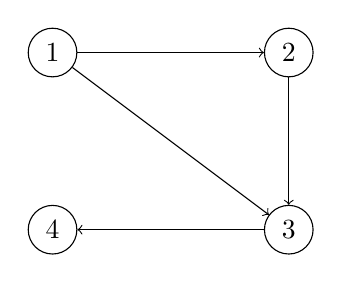
\begin{tikzpicture}[scale=3]
						\tikzstyle{vertex}=[circle,draw=black]
						\node[vertex](v1) at (0,0.75) {1};
						\node[vertex](v2) at (1,0.75) {2};
						\node[vertex](v3) at (1,0) {3};
						\node[vertex](v4) at (0,0) {4};
						\draw[->](v1) -- (v2);
						\draw[->](v1) -- (v3);
						\draw[->](v2) -- (v3);
						\draw[->](v3) -- (v4);
					\end{tikzpicture}$$

			\end{minipage}
			\hfill
			\begin{minipage}{0.45\textwidth}
				$$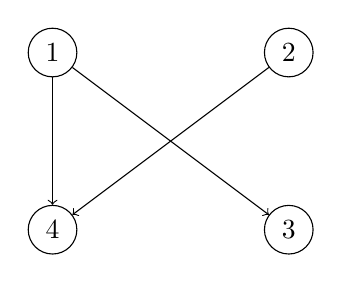
\begin{tikzpicture}[scale=3]
						\tikzstyle{vertex}=[circle,draw=black]
						\node[vertex](v1) at (0,0.75) {1};
						\node[vertex](v2) at (1,0.75) {2};
						\node[vertex](v3) at (1,0) {3};
						\node[vertex](v4) at (0,0) {4};
						\draw[->](v1) -- (v3);
						\draw[->](v1) -- (v4);
						\draw[->](v2) -- (v4);
					\end{tikzpicture}$$
			\end{minipage}
		\subsection{Matricers grafiske repræsentation}
			Her er en kant repræsentærbar ved den går fra række nummer til søjle nummer.\\
			\begin{minipage}{0.45\textwidth}
				$$\begin{bmatrix}0&1&1&0\\0&0&1&0\\0&0&0&1\\0&0&0&0\end{bmatrix}$$
			\end{minipage}
			\hfill
			\begin{minipage}{0.45\textwidth}
				$$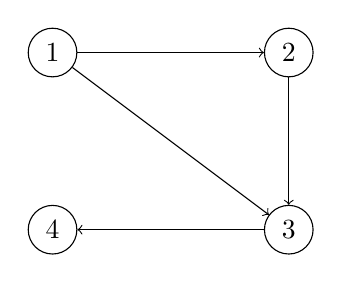
\begin{tikzpicture}[scale=3]
						\tikzstyle{vertex}=[circle,draw=black]
						\node[vertex](v1) at (0,0.75) {1};
						\node[vertex](v2) at (1,0.75) {2};
						\node[vertex](v3) at (1,0) {3};
						\node[vertex](v4) at (0,0) {4};
						\draw[->](v1) -- (v2);
						\draw[->](v1) -- (v3);
						\draw[->](v2) -- (v3);
						\draw[->](v3) -- (v4);
					\end{tikzpicture}$$
			\end{minipage}
	\section{Grafer}
		Simple grafer best[r af en mængde af knuder og kanter. Den har ingen kredse/loop og flere kanter mellem 2 knuder\\
		Orienterede grafer har en angivet kant vej.\\
		Ikke orienterede grafer st[r ud ved at et kant par kan stå i vilkårlig rækkefølge.\\
		Multigrafer er hvor der er parralelle kanter, dvs flere kanter i samme retning mellem to kanter.\\
		Dette kan både lade sig gøre på orienterede og ikke orientede grafer.\\
		Grader - antallet af kanter som ramme en knude\\
		Samlet antal grader er lig med den dobbelte mængde af kanter.
		\subsection{Terminologi}
			Del grafer kan undermængder af grafer som kan indeholde nogle af knuderne og kanter.
			Delgraf induceret er en mængde af knuder og alle kanter imellem demi
			\subsubsection{Ikke orientede grafer}
				\begin{minipage}{0.55\textwidth}
					\begin{itemize}
						\item $e_1$ forbinder d og d\\
						\item $e_1$ er incident til b og d\\
						\item $e_1$ har endepunkterne b og d\\[4mm]
						\item b og d er naboer\\
						\item b og d er adjacente\\
						\item $e_1$ og $e_2$ er adjaente\\
						\item $e_2$ og $e_3$ er parallelle\\
						\item $N(b)=\{c,d\}$ er b's nabomængde\\
						\item $N(\{b,d\})=N(b)\cup N(d)$
					\end{itemize}
				\end{minipage}
				\hfill
				\begin{minipage}{0.35\textwidth}
					$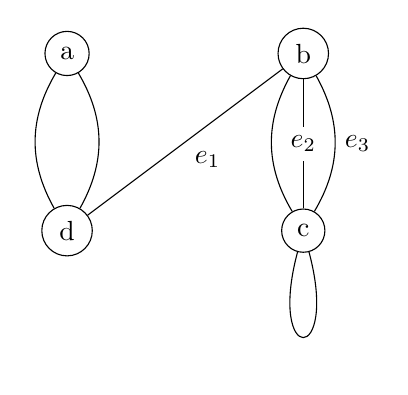
\begin{tikzpicture}[scale=3]
						\tikzstyle{vertex}=[circle,draw=black]
						\node[vertex](v1) at (0,0.75) {a};
						\node[vertex](v2) at (1,0.75) {b};
						\node[vertex](v3) at (1,0) {c};
						\node[vertex](v4) at (0,0) {d};
	   					\draw (v1) to [bend right=-30] (v4);
	   					\draw (v1) to [bend right=30] (v4);
	   					\draw (v2) to ["{$e_1$}"] (v4);
	   					\draw (v2) to [bend left=30, "{$e_3$}"] (v3);
	   					\draw (v2) to [bend right=30] (v3);
						\draw(v3) to [loop below] node {}(v3);
						\draw (v2) -- (v3) node [midway, fill=white] {$e_2$};
					\end{tikzpicture}$
				\end{minipage}
			\subsubsection{Orientede grafer}
				\begin{minipage}{0.55\textwidth}
					\begin{itemize}
						\item $e_1$ og $e_2$ er antiparallelle\\
						\item $e_1$ har startknude $a$ og slutknude $b$\\
						\item $e_1$ er incident fra $a$ og incident til $b$\\
						\item $d$ er b[de start og slutknude for $e_5$\\
						\item $deg^-(a)=1$ (indgrad)\\
						\item $deg^+(a)=1$ (udgrad)
						\item Underliggende ikke orienterede graf er grafen uden retning
					\end{itemize}
				\end{minipage}
				\hfill
				\begin{minipage}{0.35\textwidth}
					$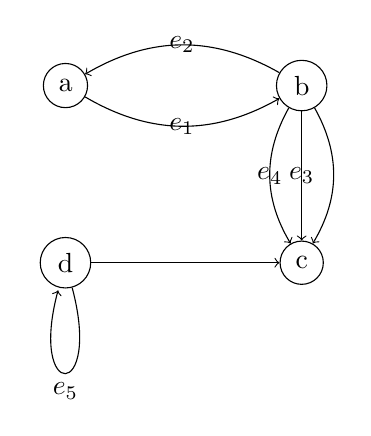
\begin{tikzpicture}[scale=3]
						\tikzstyle{vertex}=[circle,draw=black]
						\node[vertex](v1) at (0,0.75) {a};
						\node[vertex](v2) at (1,0.75) {b};
						\node[vertex](v3) at (1,0) {c};
						\node[vertex](v4) at (0,0) {d};
						\path[->]
							(v1) edge[bend right] node {$e_1$} (v2)
							(v2) edge[bend right] node {$e_2$} (v1)
							(v2) edge[] node {$e_3$} (v3)
							(v2) edge[bend left] node {} (v3)
							(v2) edge[bend right] node {$e_4$} (v3)
							(v4) edge[] node {} (v3)
							(v4) edge[loop below] node {$e_5$} (v4);
					\end{tikzpicture}$
				\end{minipage}
		\subsection{Matching}
			Matching er en mængde af ikek adjacente kanter.\\
			Maksimal matching er mængden af kanter således der ikke er andre muligheder.\\
			Maksimum matching er mængden af kanter således der er flest uden andre muligheder.\\
		\subsection{Grafklasser}
			\subsubsection{Komplette grafer}
				En graf hvor alle kanter er naboer.\\
				$k_1=
\begin{tikzpicture}[scale=3]
					\tikzstyle{vertex}=[circle,draw=black]
					\node[vertex](v1) at (0,0){};
				\end{tikzpicture}$\\
				$k_2=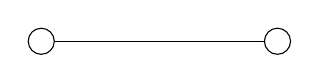
\begin{tikzpicture}[scale=3]
					\tikzstyle{vertex}=[circle,draw=black]
					\node[vertex](v1) at (0,0){};
					\node[vertex](v2) at (1,0){};
					\path[-]
						(v1) edge node {}(v2);
				\end{tikzpicture}$\\
				$k_4=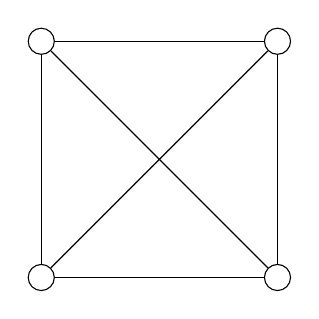
\begin{tikzpicture}[scale=3]
					\tikzstyle{vertex}=[circle,draw=black]
					\node[vertex](v1) at (0,0){};
					\node[vertex](v2) at (1,0){};
					\node[vertex](v3) at (0,1){};
					\node[vertex](v4) at (1,1){};
					\path[-]
						(v1) edge node {}(v2)
						(v1) edge node {}(v3)
						(v1) edge node {}(v4)
						(v3) edge node {}(v2)
						(v3) edge node {}(v4)
						(v4) edge node {}(v2);
				\end{tikzpicture}$\\
			\subsubsection{kredse}
				$k_3=\begin{tikzpicture}[scale=3]
					\tikzstyle{vertex}=[circle,draw=black]
					\node[vertex](v1) at (0,0){};
					\node[vertex](v2) at (1,0){};
					\node[vertex](v3) at (0.5,1){};
					\path[-]
						(v1) edge node {}(v2)
						(v2) edge node {}(v3)
						(v3) edge node {}(v1);
				\end{tikzpicture}$
				$k_4=\begin{tikzpicture}[scale=3]
					\tikzstyle{vertex}=[circle,draw=black]
					\node[vertex](v1) at (0,0){};
					\node[vertex](v2) at (1,0){};
					\node[vertex](v4) at (0,1){};
					\node[vertex](v3) at (1,1){};
					\path[-]
						(v1) edge node {}(v2)
						(v2) edge node {}(v3)
						(v4) edge node {}(v1)
						(v3) edge node {}(v4);
				\end{tikzpicture}$\\
			\subsubsection{Hjul}
				$w_3=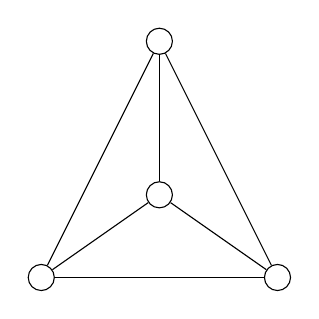
\begin{tikzpicture}[scale=3]
					\tikzstyle{vertex}=[circle,draw=black]
					\node[vertex](v1) at (0,0){};
					\node[vertex](v2) at (1,0){};
					\node[vertex](v3) at (0.5,1){};
					\node[vertex](v4) at (0.5,0.35){};
					\path[-]
						(v1) edge node {}(v2)
						(v2) edge node {}(v3)
						(v3) edge node {}(v1)
						(v4) edge node {}(v1)
						(v4) edge node {}(v2)
						(v4) edge node {}(v3);
				\end{tikzpicture}$
				$w_4=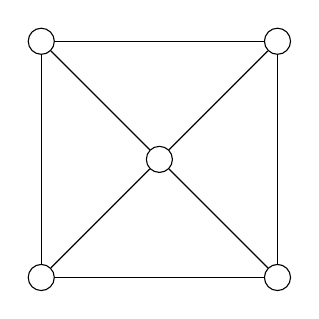
\begin{tikzpicture}[scale=3]
					\tikzstyle{vertex}=[circle,draw=black]
					\node[vertex](v1) at (0,0){};
					\node[vertex](v2) at (1,0){};
					\node[vertex](v4) at (0,1){};
					\node[vertex](v3) at (1,1){};
					\node[vertex](v5) at (0.5,0.5){};
					\path[-]
						(v1) edge node {}(v2)
						(v2) edge node {}(v3)
						(v4) edge node {}(v1)
						(v3) edge node {}(v4)
						(v5) edge node {}(v1)
						(v5) edge node {}(v2)
						(v5) edge node {}(v3)
						(v5) edge node {}(v4);
				\end{tikzpicture}$\\
			\subsubsection{Hypercubes}
				$Q_2=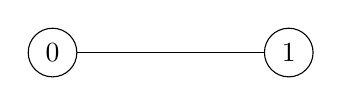
\begin{tikzpicture}[scale=3]
					\tikzstyle{vertex}=[circle,draw=black]
					\node[vertex](v1) at (0,0) {0};
					\node[vertex](v2) at (1,0) {1};
					\path[-]
						(v1) edge node {}(v2);
				\end{tikzpicture}$\\
				$Q_2=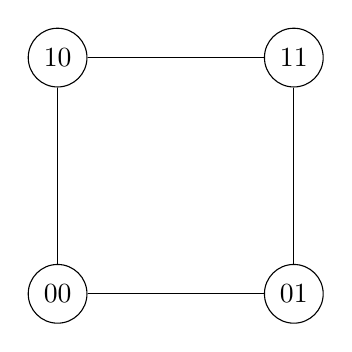
\begin{tikzpicture}[scale=3]
					\tikzstyle{vertex}=[circle,draw=black]
					\node[vertex](v1) at (0,0) {00};
					\node[vertex](v2) at (1,0) {01};
					\node[vertex](v4) at (0,1) {10};
					\node[vertex](v3) at (1,1) {11};
					\path[-]
						(v1) edge node {}(v2)
						(v2) edge node {}(v3)
						(v4) edge node {}(v1)
						(v3) edge node {}(v4);
				\end{tikzpicture}$
				$Q_3=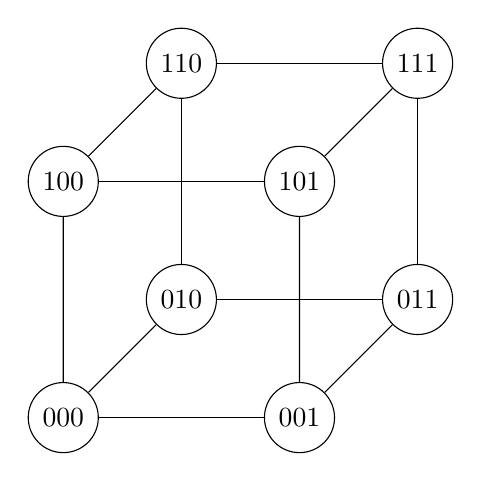
\begin{tikzpicture}[scale=3]
					\tikzstyle{vertex}=[circle,draw=black]
					\node[vertex](v1) at (0,0) {010};
					\node[vertex](v2) at (1,0) {011};
					\node[vertex](v4) at (0,1) {110};
					\node[vertex](v3) at (1,1) {111};
					\node[vertex](v5) at (0.5,-0.5) {001};
					\node[vertex](v6) at (-0.5,-0.5) {000};
					\node[vertex](v7) at (0.5,0.5) {101};
					\node[vertex](v8) at (-0.5,0.5) {100};
					\path[-]
						(v1) edge node {}(v2)
						(v2) edge node {}(v3)
						(v4) edge node {}(v1)
						(v3) edge node {}(v4)

						(v5) edge node {}(v7)
						(v6) edge node {}(v5)
						(v7) edge node {}(v8)
						(v8) edge node {}(v6)

						(v1) edge node {}(v6)
						(v2) edge node {}(v5)
						(v3) edge node {}(v7)
						(v4) edge node {}(v8);
				\end{tikzpicture}$\\
			\subsubsection{Todelte grafer}
				Todelte grafer er hvor grafen kan deles op således at 1 gruppering ikke har interne knuder men kun kanter til en anden gruppering. Dermed hvis grafen indeholder en ulige kreds kan den ikke todeles.\\
				Eks\\
				$\begin{tikzpicture}[scale=3]
						\tikzstyle{vertex}=[circle,draw=black]
						\node[vertex, color=blue](v1) at (0,0){};
						\node[vertex,color =red](v2) at (1,0){};
						\node[vertex,color=red](v4) at (0,1) {};
						\node[vertex,color=blue](v3) at (1,1) {};
						\path[-]
							(v1) edge node {}(v2)
							(v2) edge node {}(v3)
							(v4) edge node {}(v1)
							(v3) edge node {}(v4);
					\end{tikzpicture}$\\
			\subsubsection{Komplette todelte grafer}
			Grafer som er basseret på todelte grafer som gøresså komplett som muligt. Her vil grafen $K_{m,n}$ havde $m+n$ knuder og $m\cdot n$ kanter.\\	
				$K_{3,2}=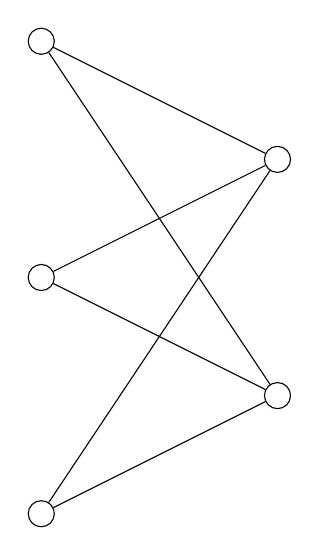
\begin{tikzpicture}[scale=3]
						\tikzstyle{vertex}=[circle,draw=black]
						\node[vertex](v1) at (0,0){};
						\node[vertex](v2) at (0,1){};
						\node[vertex](v3) at (0,2) {};
						\node[vertex](v4) at (1,0.5) {};
						\node[vertex](v5) at (1,1.5) {};
						\path[-]
							(v1) edge node {}(v4)
							(v1) edge node {}(v5)
							(v2) edge node {}(v4)
							(v2) edge node {}(v5)
							(v3) edge node {}(v4)
							(v3) edge node {}(v5);
					\end{tikzpicture}$\\
	\subsection{Repræsenation af grafer}
		\subsubsection{Adjacenslister}
			En listem ed nabo til alle punkter. Ved orienterede grafer er det punkter som den givende knude går til. Kan også repræsenteres som matricer, hvor ikke orienterede vil være symmetriske.\\
			\begin{minipage}{0.45\textwidth}
				$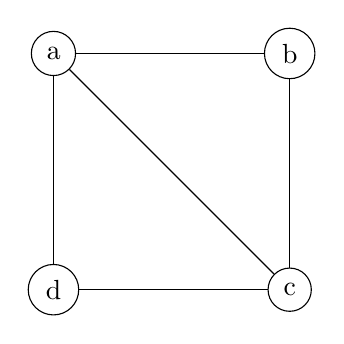
\begin{tikzpicture}[scale=3]
						\tikzstyle{vertex}=[circle,draw=black]
						\node[vertex](v1) at (0,0){d};
						\node[vertex](v2) at (1,0){c};
						\node[vertex](v4) at (0,1) {a};
						\node[vertex](v3) at (1,1) {b};
						\path[-]
							(v1) edge node {}(v2)
							(v2) edge node {}(v3)
							(v4) edge node {}(v1)
							(v3) edge node {}(v4)
							(v2) edge node {}(v4);
					\end{tikzpicture}$\\
			\end{minipage}
			\hfill
			\begin{minipage}{0.45\textwidth}
				\begin{itemize}
					\item a: b,c,d
					\item b: a,c
					\item c: a,b,d
					\item d: a,c
				\end{itemize}
			\end{minipage}	
	\subsection{Isomorfi}
		Beskriver om to grafer er ens. Tjekkes ved bijektion, hvor man mapper knuder på knuder på den anden graf således de får ens naboer på begge grafer.
	
	\subsection{Graf stier og kredse}
		Sti - en sekvens af knuder med en kant orienteret i korrekt retning, angivet i rækkefølge af knuder og længden er mængden af kanter\\
		En ikke simpel sti passere en knuder flere gange. (kan være hvis en kant blvier brugt flere gange)\\
		Kredse - stier som starter og slutter i samme knude\\
	\subsection{Graf sammenhænge}
		En graf er sammenhængende hvis der er en sti mellem ethvert par af knuder\\
		Sammenhængskomponenter er mængden af maksimal sammenhængende delgrafer. DVS mængden af steder hvor grafen adskiller delgraferne.\\
		Ved orienteret grafer så er der to typer af sammenhænge\\
		\begin{itemize}
			\item Svagt sammenhængende - Bruger underliggende graf
			\item Stærk sammenhængende - Her skal stien tage højde for orienterende
		\end{itemize}
		$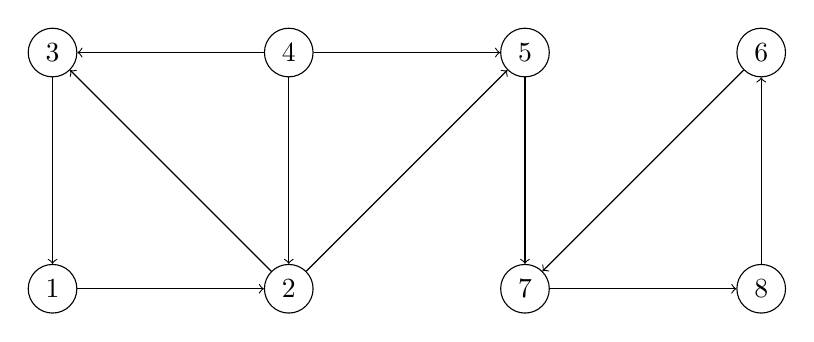
\begin{tikzpicture}[scale=3]
			\tikzstyle{vertex}=[circle,draw=black]
			\node[vertex](v1) at (0,0){1};
			\node[vertex](v2) at (1,0){2};
			\node[vertex](v4) at (0,1) {3};
			\node[vertex](v3) at (1,1) {4};
			\node[vertex](v5) at (2,1) {5};
			\node[vertex](v6) at (3,1) {6};
			\node[vertex](v7) at (2,0) {7};
			\node[vertex](v8) at (3,0) {8};
			\path[->]
				(v2) edge node {}(v5)
				(v3) edge node {}(v2)
				(v4) edge node {}(v1)
				(v3) edge node {}(v4)
				(v2) edge node {}(v4)
				(v3) edge node {}(v5)
				(v1) edge node {}(v2)
				(v5) edge node {}(v7)
				(v7) edge node {}(v8)
				(v6) edge node {}(v7)
				(v8) edge node {}(v6);
		\end{tikzpicture}$\\
		Det kan eksempelvis ses her hvordan 1,2,3,4 danner en stærk smh.komp. 5 gør også og 6,7,8 gør.\\
		Dermed er der 3 stærk smh. komp.
	\subsection{Træer}
		Ikke orienteret sammenhængende, acyklisk (ingen kreds) graf.\\
		For ethvert træ eksistere der kun én sti mellem to punkter
		\subsubsection{Bevis $G$ er et træ $\iff \forall u,v \in V: \exists !$ sti mellem $u$ og $v$}
			Pr. Def er et træ sammenhængende, dermed er der en sti mellem alle punkter\\
			Pr. Def er et træ acyklisk, som medføre at der kun kan være 1 sti, da hvis der skal være to stier påkræver det en kreds.
			Ligesådan bevis i den anden retning\\
			Hvis der altid er en sti og der ikke er mere end 1 sti er den sammenhængende og acyklisk\\
			Dette er def. på et træ.
		\subsubsection{Et træ med $n$ knuder har altid $n-1$ kanter}
			Induktionsbevis\\
			Basis $n=1$ roden har ingen kanter\\
			Ind.ant $n=k\geq 1$\\
			Ind. skridt: Ved tilføjelsen af en knude på en rod eller anden knude vil det give 1 kant
\section{Følger}
	Sequence/Følge en ordnet mængde. Eks. fibonacci-tallene\\
	Notation:
		$$a_n=\frac{1}{n},\; n\geq 1$$
	For dette vil $\{a_n\}$ betyde hele følgen.\\
	\subsection{Geometrisk følge}
		Følger som går ud fra formen $a_n=cr^n$, $n\in \mathbb{N}$\\
		Her er $c$ begyndelsesled og $r$ er fælles faktor\\
		Eks for den rekursive def. $a_0=1$, $a_n=\frac{1}{2}\cdot a_{n-1}$ vil den være $a_n=1\cdot \frac{1}{2}^n$
	\subsection{Aritmestisk følge}
		$a_n=b+nd$ $b$ begyndelsesled og $d$ fælles forksel.\\
		eks. $1,3,5,7$ vil $b=1$ og $d=2$
	\subsection{Mandelbrot-fraktalen}
	def: $x_0=0$, $x_n=x^2_{n-1}+c$ hvor $c$ er et kompleks tal\\
	Hvis følgen er begrænset er $c$ en del af mandelbrot mængden.\\
	Hvis $|x_n|>2$ vil den ikke v;re begr;nset og kaldes Escape condition og desto hurtigere det opnåes vil det illustreres ved at være lysere.
	\subsubsection{$i$ tilhøre Mandelbrot mængden}
		\begin{align*}
			x_0&=0\\
			x_1&=0^2+i=i\\
			x_2&=i^2+i=-1+i &&i=\sqrt{-1}\rightarrow i^2=-1\\
			x_3&=(-1+i)^2+i=1-1-2i+i=-i\\
			x_4&=(-i)^2+i=-1+i\\
			x_5&=x_3
		\end{align*}
		Dermed er mængden begrænset og en del af mandelbrot mængden. Det vil blive vist ved det komplekse tal er y komponenten dermed er dette (0,1) koordinatet. Dermed er kooridnatet sort
\section{Rækker}
	Rækker er sum af et (uendeligt) antal led.
	\subsection{Eksempel $1+\frac{1}{2}+\frac{1}{4}+\frac{1}{8}+...$}
		\begin{align*}
			n&=0: &&1=2-1\\
			n&=1: &&1+\frac{1}{2}=2-\frac{1}{2}\\
			n&=2: &&1+\frac{1}{2}+\frac{1}{4}=2-\frac{1}{4}\\
			n&=3: &&1+\frac{1}{2}+\frac{1}{4}+\frac{1}{8}=2-\frac{1}{8}\\
			n&=n: &&\sum\limits_{i=0}^n(\frac{1}{2})^n=2-(\frac{1}{2})^n\\
			n&=\infty: &&\sum\limits_{i=0}^\infty (\frac{1}{2})^n=2
		\end{align*}
	\subsection{Summation af rækker}
		\begin{align*}
			\sum\limits_{k=0}^n&ar^k(r\neq 0) &&\frac{ar^{n+1}-a}{r-1}, r\neq 1\\
			\sum\limits_{k=1}^n&k &&\frac{n(n+1)}{2}\\
			\sum\limits_{k=1}^n&k^2 &&\frac{n(n+1)(2n+1)}{6}\\
			\sum\limits_{k=1}^n&k^3 &&\frac{n^2(n+1)^2}{4}\\
			\sum\limits_{k=1}^\infty&x^k,|x|<1 &&\frac{1}{1-x}\\
			\sum\limits_{k=1}^n&x^{k-1},|x|<1 &&\frac{1}{(1-x)^2}\\
		\end{align*}
	\subsection{Geometriske række}
		$\sum\limits_{i=0}^nar^i$
		Det ses her at hvis man sætter $(r-1)$ får man:\\
		\begin{align*}
			(r-1)\sum\limits_{i=o}^nr^i&=(r-1)(r^0+r^1+...r^n)\\
						   &=r^=r^2+...+r^{n+1}-(r^0+r^1+...r^n)\\
						   &=r^{n+1}-r^0\\
			\sum\limits_{i=0}^nr^i&=\frac{r^{n+1}-1}{r-1}
		\end{align*}
		Her blev begyndelsesledet undladt da det blot kan sættes på efterfølgende.
		For $r=i$ vil det blot gælde at $\sum\limits_{i=0}^nr^i=n+1$
	\subsection{Artmetisk række}
		$\sum\limits_{i=0}^n(b+id)$\\
		Genrealt kan det findes at:
		\begin{align*}
			\sum\limits_{i=0}^n(b+id)&=\sum\limits_{i=0}^nb+\sum\limits_{i=0}^nid\\
						 &=\sum\limits_{i=0}^nb+d\sum_{i=0}^ni\\
						 &=(n+1)b+d\\
						 &=\frac{n(n+1)}{2}
		\end{align*}
		Den sidste omskrivning kommer ved at hvis man udleder udtrykket ses det at der dannes parvis led bortset fra det sidste og det første som er lig med $\frac{n(n+1)}{2}$
		\subsubsection{Eksempel $1+3+5+..+2k-1$}
			$\sum\limits_{i=0}^{k-1}1+2i=k+(k-1)k=k^2$
	\subsection{Rækker i loops}
		Det kan også bruges til at finde antal gennemgang i for loops:\\
		eks. 
		\begin{lstlisting}
for i=1 to 20
	for j=1 to i
		...
		\end{lstlisting}
		Dette vil køre $\frac{20(20+1)}{2}=210$ gange\\
		Ved summer som starter højere kan det omskrives\\
		$\sum\limits_{i=11}^{20}i=\sum\limits_{i=1}^{20}i-\sum\limits_{i=1}^{10}i$\\
		For 3 nested loops:
		\begin{lstlisting}
for i=1 to 20
	for j=1 to i
		for k=1 to j
		\end{lstlisting}
		Vil den køre 
		\begin{align*}
			\sum\limits_{i=1}^{20}\sum\limits_{j=1}^ij&=\sum\limits_{i=1}^{20}\frac{i(i+1)}{2}\\
								  &=\frac{1}{2}(\sum\limits_{i=1}^{20}(i^2+i))\\
								  &=\frac{1}{2}(\sum\limits_{i=1}^{20}i^2+\sum\limits_{i=1}^{20}i)\\
								  &=\frac{1}{2}(\frac{20\cdot 21\cdot 41}{6}+\frac{20(20+1)}{2})\\
								  &=1540
		\end{align*}
		Ved $i^2$ kunne en tabel fra s.176 i bogen bruges.
	\subsection{Notation}
		$\sum\limits_{i=1}^{n}i=\sum\limits_{i\leq i\leq n}i=\sum\limits_{i\in A}i,$ hvor $A=\{1,2,3,...,n\}$
	\subsection{Uendelige rækker}
		For den uendelige række $\sum\limits_{n=1}^{\infty}a_n$, vil $s_n=\sum\limits_{n=1}^{\infty}a_i$ være den n'te partielle sum.\\
		hvis $\exists s\in \mathbb{R}: \lim\limits_{n\rightarrow \infty}s_n=s$ siges det at rækken konvergere mod $s$\\
		Dvs. at hvis en partiel række af en uendelig række konvergere, vil den uendelige række konvergere.\\
		Ligesådan må kan også gerne starte på et vilkårligt punkt for at undersøge om rækken konvergere\\[4mm]
		Hvis en ultimativ positiv følge er begrænset ovenfra vil den altid konvergere, da den aldrig vil blive negativ og blot nå det begrænset punkt og konvergere.\\
		Hvis $\sum\limits_{n=1}^{\infty}a_n=A$ og $\sum\limits_{n=1}^{\infty}b_n=B$ da gælder:
		\begin{itemize}
			\item $\sum\limits_{n=1}^{\infty}ca_n=cA$
			\item $\sum\limits_{n=1}^{\infty}(a_n+b_n)=A+b$
			\item $a_n\leq b_n \rightarrow A\leq B$, for alle $n\geq 1$
		\end{itemize}
		
			Dermed er den harmoniske serie divergerende, da integralet bliver uendeligt.
	
		
\section{Følger og konvergens}
	\subsection{Notation}
		Hvis $a_n \geq L$ for $n\in\mathbb{N}^+$ siges:
		\begin{itemize}
			\item $\{a_n\}$ er begrænset nedera fra $L$
			\item $L$ er en nedre grænse for $\{a_n\}$
		\end{itemize}
		Hvis $a_n \leq M$ for $n\in\mathbb{N}^+$, siges:
		\begin{itemize}
			\item $\{a_n\}$ er begrænset ovenfra af $M$
			\item $M$ er en øvre grænse for $\{a_n\}$
		\end{itemize}
		Hvis $\{a_n\}$ er begrænset både ovenfra og nedenfra er den bægrenset.\\[4mm]
		Hvis alle elementer er større eller lig med 0 er den positiv\\
		Hvis den er mindre eller lig med 0 er den negativ.\\
		Hvis alle elementer $a_{n+1}\geq a_n$ er den voksende\\
		Hvis alle elementer $a_{n+1}\leq a_n$ er den aftagende\\
		Hvis ikke den vokser eller aftager er den monoton\\
		hvis alle elementer $a_na_{n=1}<0$ er den alternerende, dvs skiftende mellem positiv og negativ
	\subsection{Konvergens}
		Hvis en række går mod en given værdi når rækken bliver uendelig.\\
		$\forall \epsilon > 0: \exists N \in \mathbb{Z}:\forall n \geq N: |a_n-L|<\epsilon$\\
		Dvs. for alle værdier $\epsilon$ som er større end 0, vil der eksistere et punkt i rækken hvor alle efterfølgende punkter vil være mindre end alle $\epsilon$ værder. Grænseværdien $L$ bliver her bare brugt hvis et tal konvergere til 1, vil $L=1$.\\
		$\lim\limits_{n\rightarrow\infty} a_n=L$
		Eks. $\{\frac{n-1}{n}\}=0,\frac{1}{2},\frac{2}{3},...$ vil konvergere mod 1\\[4mm]
		Hvis $\sum\limits_{n=1}^{\infty}a_n$ konvergere vil det sige at $\lim\limits_{n\rightarrow \infty}a_n=0$\\
		Det kan ses da $\lim\limits_{n\rightarrow \infty}a_n=\lim\limits_{n\rightarrow\infty}(S_n-S_{n-1})$ som medføre ud fra sætningen $\lim\limits_{n\rightarrow \infty}a_n=S-S=0$\\
		Kan bruges ved eks $\sum\limits_{n=1}^{\infty}\frac{n}{2n-1}$ hvor brøkken er $a_n$ hvor grænseværdien er $\frac{1}{2}$ og dermed divigere det originale udtryk mod uendeligt\\[4mm]
		Hvis en række konvergere, vil man kunne undlade start og slut af en række.
	\subsection{Konvergen kriterier}
		\subsubsection{Sammenlignings-kriteriet}
			Hvis $0\geq a_n \geq K\cdot b_n$ ultimativt, vil det gælde at:
			\begin{itemize}
				\item $\sum\limits_{n=1}^{\infty}b_n$ (konv.) $\rightarrow \sum\limits_{n=1}^{\infty}a_n$ (konv.)\\
				\item $\sum\limits_{n=1}^{\infty}a_n = \infty$ (div.) $\rightarrow \sum\limits_{n=1}^{\infty}b_n=\infty$ (div.)
			\end{itemize}
			Det kan nemlig ses at det første udtryk, egentlig blot er definiationen på konvergens, og det andet udtryk er egentlig det første udtryk negeret.\\
			Eks. $\sum\limits_{n=1}^{\infty}\frac{4}{2^n+1}$ kan sammenlignes med $\sum\limits_{n=1}^{\infty}\frac{1}{2^n}$, hvor det andet udtryk er større eller lig med når der multipliceres med en konstant her 4\\
			Her vides det at det andet udtryk konvergere, og dermed vil det første udtryk konvergere.\\
			Ligesådan vil $\sum\limits_{n=2}^{\infty}\frac{1}{\ln n}$ divergere, da $\sum\limits_{n=2}^{\infty}\frac{1}{n}$ divergere og er mindre.
		\subsubsection{Grænse-sammenlignings-kriteriet}
			Bygger på grænseværdien og tjekker om en konstant eksistere.\\
			Hvis $\{a_n\}$ og $\{b_n\}$ er positive følger og $\lim\limits_{n\rightarrow \infty}\frac{a_n}{b_n}=L$ da gælder:	
			\begin{itemize}
				\item $(L<\infty$ og $\sum\limits_{n=1}^{\infty}b_n$ konv.) $\rightarrow \sum\limits_{n=1}^{\infty}a_n$ konv.
				\item $(L > 0 $ og $\sum\limits_{n=1}^{\infty}b_n=\infty) \rightarrow \sum\limits_{n=1}^{\infty}a_n=\infty$
			\end{itemize}
			Bevis bygger på omskrivning af sammenlignings-kriteriet, hvor $L$ er en isolering af $k$\\
			Eks. $\sum\limits_{n=1}^{\infty}\frac{2n^2-3n+1}{5n^3+4n^2}$ sammenlignes med harmoniske række $\sum\limits_{n=1}^{\infty}\frac{1}{n}$\\
			Dermed bliver $\lim\limits_{n\rightarrow \infty}\frac{\frac{2n^2-3n+1}{5n^3+4n^2}}{\frac{1}{n}}=\lim\limits_{n\rightarrow \infty}\frac{2n^3-3n^2+n}{5n^3+4n^2}=\frac{2}{5}=L$\\
			Således vil eksemplet divigere, da sammenligningen divigere og $L>0$
		\subsubsection{Kvotient-kriteriet}
			Hvis en ultimativ række, hvor $\rho=\lim\limits_{n\rightarrow\infty}\frac{a_{n+1}}{a_n}$ vil det gælde at:
			\begin{itemize}
				\item $0\geq \rho < 1 \rightarrow \sum\limits_{n=1}^{\infty}a_n$ konvergere
				\item $\rho > 1 \rightarrow \lim\limits_{n\rightarrow \infty}a_n=\sum\limits_{n=1}^{\infty}a_n=\infty$
				\item $\rho = 1$ ingen information
			\end{itemize}
		\subsubsection{Konvergens kritiere for ultimative positive rækker}
		Hvis $a_n=f(n)$ hvor f er positiv, kontinuert og aftagende, vil integralet af funktionen enten divigere eller konvergere og ligesådan vil $\sum\limits_{n=1}^{\infty}a_n$ dividere eller konverger ens med funktionen.\\
		Dette kan bevises ved at lave en nedre grænse for integralet som er summen af $a_n$ fra n+1 og øvre grænse af summen $a_n$ fra n\\
		\subsubsection{Harmoniske rækker / divigerns \& konvergens test}
			Den harmoniske serie er beskrevet som $\sum\limits_{i=1}^n\frac{1}{i}$\\
			Det kan her ses at divergens test viser $\lim\limits_{n\rightarrow \infty}\frac{1}{n}=0$ dermed kan det ikke siges om den konvergere eller divigere. Hvis det gav over 0 ville det vides at den divergere.\\
			Det kan dog ses ved en integral test at integralet konvergere og såldes må serien også konvergere eller ligesådan ved divigering\\
			\begin{align*}
				\int_1^{\infty}\frac{1}{x}dx=\lim\limits_{a\rightarrow \infty}\ln x|^a_1\\
				\lim\limits_{a\rightarrow \infty}\ln a-\ln 1 = \infty - 0 = \infty
			\end{align*}
	\subsection{Divergens}
		Divergering er hvis en række ikke divigere.\\
		En række kan mere specifikt divigere mod $\infty$ eller $-\infty$
		Eks. $\{(-1)^n\}=-1,1,-1,1,...$ vil blot divigere
	\subsection{p-rækker}
		$\sum\limits_{n=1}^{\infty}\frac{1}{n^P}$\\
		Hvis $P\leq 1$ divergere mod $\infty$\\
		Hvis $P>1$ konvergere.\\
		\subsubsection{bevis}
			$P\leq 1$
			\begin{align}
				n^P\leq n\\
				\frac{1}{n^P}\geq \frac{1}{n}\\
				\sum\limits_{n=1}^{\infty}\frac{1}{n^P}=\infty
			\end{align}
			(3) da $\sum\limits_{n=1}^{\infty}\frac{1}{n}=\infty$ og da $\frac{1}{n}\geq \frac{1}{n^P}$\\
			$P>1$
			\begin{align}
				\sum\limits_{n=1}^{\infty}\frac{1}{n^P}\\
				\int_1^{\infty}\frac{1}{x^P}dx&=\int_1^\infty x^{-P}dx\\
									&=[\frac{x^{-P+1}}{1-P}]^{\infty}_1\\
									&=\lim\limits_{x\rightarrow \infty}\frac{x^{1-P}}{1-P}+\frac{1}{1-P}\\
									&=0+\frac{1}{1-P}
			\end{align}
			Da det vides at integralet for $\frac{1}{1-P}$ vil konvergere vil P-rækken også konvergere.

	\subsection{Regneregler for grænseværdi}
		\begin{itemize}
			\item $\lim\limits_{n\rightarrow\infty}(a_n+b_n)= \lim\limits_{n\rightarrow\infty} a_n + \lim\limits_{n\rightarrow\infty} b_n$\\
			\item  $\lim\limits_{n\rightarrow\infty}(a_n-b_n)= \lim\limits_{n\rightarrow\infty} a_n - \lim\limits_{n\rightarrow\infty} b_n$\\
			\item  $\lim\limits_{n\rightarrow\infty}(a_n\cdot b_n)= \lim\limits_{n\rightarrow\infty} a_n \cdot \lim\limits_{n\rightarrow\infty} b_n$\\
			\item  $\lim\limits_{n\rightarrow\infty}(\frac{a_n}{b_n})= \frac{\lim\limits_{n\rightarrow\infty} a_n}{ \lim\limits_{n\rightarrow\infty} b_n}$
			\item $\lim\limits_{n\rightarrow \infty}c\cdot a_n = c\cdot \lim\limits_{n\rightarrow\infty}a_n$
		\end{itemize}
		Eks.
		\begin{align*}
			\lim\limits_{n\rightarrow\infty}\frac{2n^2-n-1}{5n^2+n-3}\\
			\lim\limits_{n\rightarrow\infty}\frac{2-\frac{1}{n}-\frac{1}{n^2}}{5+\frac{1}{n}-\frac{3}{n^2}}\\
			\frac{\lim\limits_{n\rightarrow\infty}2-\frac{1}{n}-\frac{1}{n^2}}{\lim\limits_{n\rightarrow\infty}5+\frac{1}{n}-\frac{3}{n^2}}\\
			\frac{2-0-0}{5+0+0}\\
			\frac{2}{5}
		\end{align*}
		$\lim\limits_{n\rightarrow\infty}x^n=0$, hvis $|x|<1$\\
		\subsubsection{Bevis}
			\begin{align}
				\forall \epsilon > 0: \exists N \in \mathbb{Z}^+:\forall n\geq N: |x^n|<\epsilon\\
				|x^n|<\epsilon\\
				|x|^n<\epsilon\\
				n\ln|x|<\ln\epsilon\\
				n>\frac{\ln\epsilon}{\ln|x|}\\
				N=\rfloor\frac{\ln\epsilon}{\ln|x|}\lfloor+1\\
			\end{align}
				Det sidste del af udtrykket kan omskrives og det ses at ved det sidste $\ln|x|$ bliver divideret vender relationstegnet, da det er negativt.\\
				Det kan ud fra dette beskrives at $N$ kan være den givende værdi og det dermed eksistere således at den altid vil konvergere mod 0.\\
				Hvis $x$ er 0 gælder beviset ikke men er ikke nødvendigt da det allerede er 0 fra starten\\
				Dette giver også god mening at brøkker mindre end 1 vil efter nok gange multiplciering går mod 0.
		$\lim\limits_{n\rightarrow\infty}\frac{x^n}{n!}=0$, for alle $x\in\mathbb{R}$
		\subsubsection{Bevis}
			Da $n!$ er hurtigere voksende end $x^n$ vil det altid gå mod 0.\\
			Selv hvis $x=\infty$ vil den stadig bliver mindre da $\infty !$ er større og dermed vil den gå mod 0.
	
	



		
						
	\end{document}
		

